\documentclass[twoside,twocolumn,a4paper]{article}

\usepackage[latin1]{inputenc}
\usepackage[T1]{fontenc}
\usepackage{mathptmx}
\usepackage{graphicx}
\usepackage{estylf_en}

% In order to work with mathematical environments (propositions, theorems, etc.), the following packages are suggested:
%\usepackage{amsmath,amsthm}
\usepackage{amsmath, amsthm}
\usepackage{amsfonts}

\hyphenation{pro-per-ties}
\hyphenation{ge-ne-ral-ly}
\hyphenation{pre-fe-ren-ces}
\hyphenation{u-sing}
\hyphenation{pu-nish-ment}

\newcommand{\Pow}{\mathcal{P}}
\newcommand{\N}{\operatorname{N}}
\newcommand{\bool}{\operatorname*{\mathcal{B}}}
\newcommand{\Pos}{\operatorname{Pos}}
\newcommand{\Nec}{\operatorname{Nec}}
\newcommand{\T}{\mathcal{T}}

\begin{document}

\title{Possibilistic evaluation of fuzzy temporal intervals}

%*******************************************************
% REMARKS ABOUT THE AUTHORS
%*******************************************************
% In order to write the name and surname of an author in the the same line, the symbol ~ will be required.
%*******************************************************
% If all the authors share the same affiliation, the following commands are suggested to avoid the superscript:
% \author{Name1~Surname1}
% \address{Address1}{autor1@e-mail1.com}
%*******************************************************

\author[1]{Jos\'e Enrique~Pons}
\author[2]{Antoon~Bronselaer}
\author[1]{Olga~Pons}
\author[2]{Guy~De Tr\'e}
\address[1]{Department of Computer Science and Artificial Intelligence,University of Granada, Spain}{\{jpons,opc\}@decsai.ugr.es}
\address[2]{Department of Telecommunications and Information Processing, Ghent University, Belgium}{\{Antoon.Bronselaer,Guy.De.Tre\}@telin.ugent.be}

\maketitle

\begin{abstract}
Possibility theory tries to quantify the uncertainty caused by incomplete information. A specific case of incomplete information is that of ill-known temporal intervals. The study of these fuzzy intervals is of particular interest in temporal database research. In order to optimize the storage of fuzzy temporal intervals, some transformations have been proposed. In this paper we analyze the possibilistic evaluation of the ill-known temporal intervals and the proposed transformations. It is shown how the reasoning behind the transformations implies a possibilistic information lost. 

\textbf{Keywords:} Possibility theory, ill-known values, ill-known sets, intervals, temporal databases.\vspace{9mm}
\end{abstract}

\section{INTRODUCTION}

The connection of possibility theory \cite{Zadeh78},\cite{Shackle61},\cite{Gaines75} and fuzzy sets has been studied among others by Zadeh \cite{Zadeh65}. This connection establishes two different natures for a fuzzy set \cite{Dubois97}:
\begin{itemize}
\item
\textbf{Conjunctive nature}: The fuzzyfication of a regular set. This interpretation corresponds with the following two semantics: \textit{Degree of preference} and \textit{degree of similarity}.
\item
\textbf{Disjunctive nature}: In this case, the disjunctive nature indicates a description of incomplete knowledge. This interpretation corresponds with the semantics for the \textit{degree of uncertainty}.
\end{itemize}

The disjunctive nature can be seen as an additional connection between fuzzy set theory and possibility theory. Dubois and Prade \cite{Dubois88b} have studied the problem of inferring uncertainty about sets from uncertainty about values. They explain how the incomplete knowledge about a set can be represented as a possibility distribution over a universe $\Pow \left(U \right)$, the power set over the universe $U$. The main drawback of the approach is the large overhead that such a distribution introduces.  A mechanism for the propagation of uncertainty about set elements towards uncertainty about sets is introduced in \textit{'Possibilistic evaluation of sets'} \cite{Pon11}.

There are several proposals in the literature for inferring uncertainty about sets from uncertainty about values. It is of particular interest for fuzzy temporal databases, the application on temporal intervals. The transformation from two ill-known temporal points to a ill-known set has been discussed in \cite{Garrido2009}. In this work we will analyze the major pitfalls of these approaches and the benefit of using the mechanism proposed in \cite{Pon11}.

The paper is organized as follows. In Section \ref{sec:preliminaries}, some preliminaries and concepts about the possibilistic evaluation framework and the temporal databases are presented. The proposal for interval evaluation is done in Section \ref{sec:interval-eval}. In Section \ref{sec:analysis}, the analysis among the different transformations is done. Finally, Section \ref{sec:conclusions} presents the main conclusions and some lines for the future work in this research.


\section{\label{sec:preliminaries}PRELIMINARIES}
In this section we will introduce some basic concepts. First of all, an introduction to possibility theory is explained. Then, the concepts of fuzzy numbers and fuzzy intervals introduced by Dubois and Prade \cite{Dubois1983} are discussed. Finally, a brief introduction to temporal databases is done.

\subsection{\label{subsec:possibilistic-variables}Possibilistic variables}
A possibilistic variable $X$ over a universe $U$ is defined as a variable taking exactly one value in $U$, but for which this value is (partially) unknown. The possibility distribution $\pi_X$ gives the available knowledge about the value that $X$ takes. For each $u\in U$, $\pi_X(u)$ represents the possibility that $X$ takes the value $u$.

It is important to understand the difference between the following two concepts:
\begin{itemize}
\item
A \emph{possibilistic variable} $X$ is bounded to take only one value , but this value is not known due to incomplete knowledge. 
\item
An \emph{ill-known set}~\cite{Dubois88b}: a possibilistic variable defined over the universe $\Pow(U)$.
\end{itemize}

Note that while a possibilistic variable refers to one (partially) unknown value, an ill-known set is a crisp set but, for some reason, (partially) unknown.


\subsection{\label{subsec:fuzzy-numbers}Fuzzy numbers and fuzzy intervals}
Dubois and Prade~\cite{Dubois1983} proposed the following definition of \emph{fuzzy interval}.
%\begin{definition}
A fuzzy interval is a fuzzy set $M$ on the set of real numbers $\mathbb{R}$ such that:
\begin{eqnarray}
\forall (u,v)\in\mathbb{R}^2:&\\
\nonumber
\forall w \in [u,v]:&\mu_M(w) \geq\min(\mu_M(u),\mu_M(v))  \\
\exists m \in \mathbb{R}:& \mu_M(m)=1 
\end{eqnarray}
%\end{definition}
If $m$ is unique, then $M$ is referred to as a \emph{fuzzy number}, instead of a \emph{fuzzy interval}. In other words, if the core of a fuzzy interval is a singleton, it can be seen as a fuzzy number. In their work, Dubois and Prade propose four different functions (two possibility and two necessity functions) to asses the position of a fuzzy number N relative to  a fuzzy number M taken as a reference.

The most convenient representation for the membership function of a fuzzy number is a triangular function. The membership function $\mu_M$ for the fuzzy set $M$ has also the properties of convexity and normalization. Three values represent a triangular function (see Figure~\ref{fig:triangular}):
\begin{itemize}
\item
$D$ is the singleton value in the core of $\mu_M(x)$.
\item
$D-a$ is the lower value in the support of $\mu_M(x)$. 
\item
$D+b$ is the upper value in the support of $\mu_M(x)$.
\end{itemize}
Note that the values $a$ and $b$ are values in the underlying ordered domain. E.g. $(a,b) \in \mathbb{R}^2$. The notation for a triangular function adopted here is $[D,a,b]$.
\begin{figure}[h!]
  \centering
  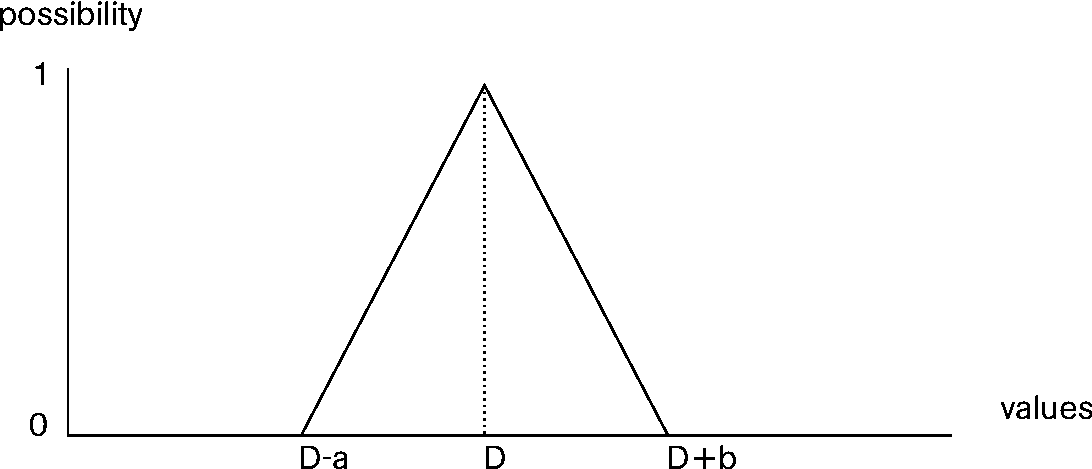
\includegraphics[scale=0.4]{graphs/triangular.pdf}
  \caption{Triangular function.}
  \label{fig:triangular}
\end{figure}

The most simple representation for the membership function of a fuzzy interval is a trapezoidal function. This membership function $\mu_T$ for the fuzzy interval $T$ is convex and normalized. Four values represent a trapezoidal membership function (figure  \ref{fig:trapezoidal}): $\left[\alpha,\ \beta,\ \gamma,\ \delta\right]$. The membership function is given by:

\begin{align}
\mu_T(x)
\begin{cases}
1 & \mbox{ if } x \in [\beta,\gamma] \\
0 & \mbox{ if } x > \delta \vee x < \alpha \\
\frac{x-\alpha}{\beta - \alpha} & \mbox{ if } x \in [\alpha,\beta[ \\
\frac{\delta -x}{\delta - \gamma} & \mbox{ if } x \in ]\gamma,\delta] \\
\end{cases}
\end{align}

\begin{figure}[h!]
  \centering
  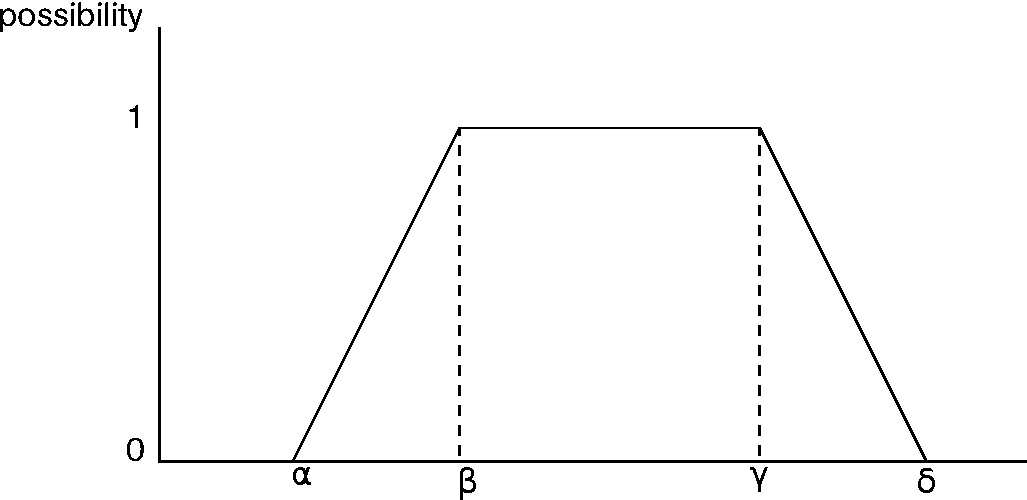
\includegraphics[scale=0.4]{graphs/trapezoidalDistribution.pdf}
  \caption{Trapezoidal distribution.}
  \label{fig:trapezoidal}
\end{figure}



\subsection{\label{subsec:temporal}Temporal databases}
%In this section, the proposed reasoning is applied to the specific context of intervals on the real line. This setting is of specific interest in the context of fuzzy temporal databases.
A temporal database \cite{Dyreson1994} is a database that manages some aspects of time in its schema. A \textbf{chronon} is the shortest duration of time supported by the database. The time can be represented either as points or intervals \cite{655777}. Fuzzy temporal models \cite{4481150} are proposed when the time points or intervals are not precisely known. There are proposals for the  fuzzyfication of the time point \cite{Dubois89} and the fuzzyfication of the time interval \cite{Garrido2009}.\\
Allen \cite{Allen:1983:MKT:182.358434} studied the comparison between two crisp time intervals. For fuzzy intervals, several proposals \cite{4481150}, \cite{springerlink:10.1007/978-3-540-39964-3_57},\cite{10.1109/TIME.2004.1314418} have been done.


%Time granularity is also associated with the representation of the time. A granularity is the result of partitioning on the set of chronons. The conversion among granularities is a common issue within temporal databases \cite{Lin97efficientconversion}. Granularity is the basis of some systems \cite{Cru97},\cite{624013}.


Despite of user-defined time (an uninterpreted attribute; supported in the standard SQL2 \cite{Mel93}), there are 3 types of time in a temporal database:

\begin{itemize}
	\item
	\textbf{Transaction time}: The time when the fact is stored in the database.
	\item
	\textbf{Valid time}: The time when the fact is true in the modelled reality.
	\item
	\textbf{Decision time} \cite{Nascimento95decisiontime}: The time when an event was decided to happen. 
	\end{itemize}
	
	 The  database model can be then classified into: transaction time \cite{Ston87},\cite{Jensen:1991:IIM:627283.627484}, Valid time, bi-temporal \cite{Snodgrass:1984:TQL:588011.588041}(both valid and transaction time) or tri-temporal \cite{Nascimento95decisiontime} (valid, transaction and decision time).

Fuzzy temporal models \cite{4481150} deal with time points \cite{Dubois89} or intervals \cite{Garrido2009} that are ill-known. Some fuzzy temporal models assume that the time stored in the database is an interval. The temporal interval is represented by two ill-known time points: $X$  an ill-known starting point and $Y$ an ill-known ending point. The interval $\left[X,Y\right]$ is not a fuzzy interval but an ill-known interval: it is a crisp interval but it is partially unknown which values are in this interval.



% In such databases, points in time can be ill-known, i.e. the starting, the ending or both points are ill-known. a point in time is modelled as an ill-known value. When two such ill-known points are given, an interesting problem is the inference of uncertainty about the interval that is enclosed by these two ill-known points. In the proposed framework, this problem can be solved by evaluating an interval against two ill-known constraints, where the binary relations are ordering relations on the set of real numbers.

\section{\label{sec:interval-eval}INTERVAL EVALUATION BY ILL-KNOWN CONSTRAINTS}
The problem of the interval evaluation is explained in \cite{Pon11}: For a crisp interval $I = \left[ a, b \right]$, we want to know if all points in this interval reside between the boundaries of the ill-known interval $\left[ X , Y \right]$, where $X,Y$ are ill-known values on the set of real numbers $\mathbb{R}$, and $\lambda$ is the evaluation function. The following expressions compute the possibility and the necessity: 

\begin{eqnarray}
\label{eq:interval-pos}
\Pos\left(\lambda([a,b])\right)=\\
\nonumber
\min\bigg(\sup_{a\geq w}\pi_{X}(w),\sup_{b\leq w}\pi_{Y}(w)\bigg)\\
\label{eq:interval-nec}
\Nec\left(\lambda([a,b])\right)=\\
\nonumber
\min\bigg(\inf_{a<w}1-\pi_{X}(w),\inf_{b>w}1-\pi_{Y}(w)\bigg).
\end{eqnarray}

\paragraph{Example} Consider the ill-known values $X = \left[5, 2, 8\right]$ and $Y = \left[9, 7, 10 \right]$. The knowledge about the evaluation of the interval $\left[a, b \right]$  is given by the expressions \eqref{eq:interval-pos},\eqref{eq:interval-nec}.  Figure~\ref{fig:3d-possibility} shows a 3D plot of the possibility that an interval $[a,b]$ passes the evaluations specified by the ill-known constraints. Note the triangular form for the resulting possibility distribution since the condition $a \leq b$ holds.

\begin{figure}[h!]
\centering
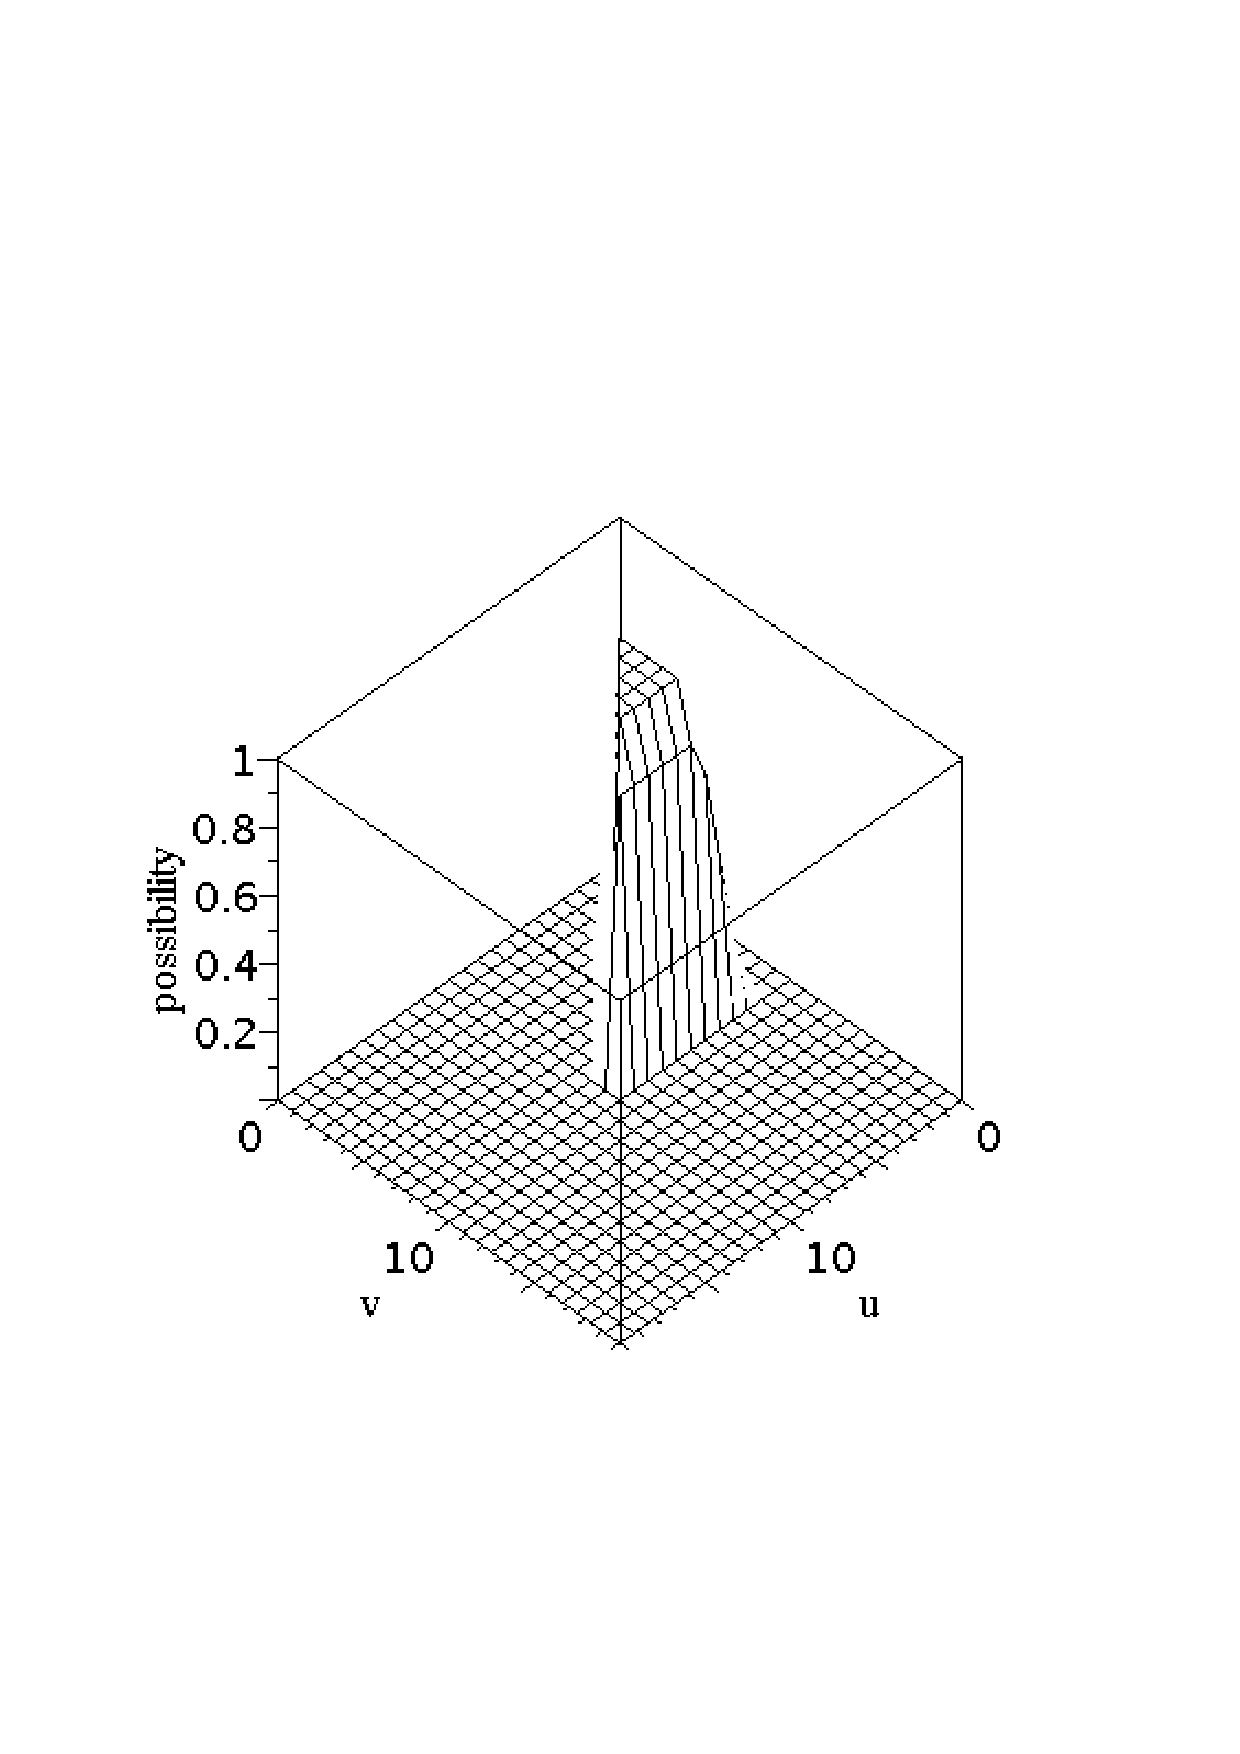
\includegraphics[scale=0.4]{graphs/3D_possibility.pdf}
\caption{Possibility of evaluation for the interval $[a,b]$.}
\label{fig:3d-possibility}
\end{figure}
The necessity plot is obtained in a similar way and is shown in Figure~\ref{fig:3d-necessity}. Notice that the necessity measure is not normalized because the supports of $X$ and $Y$ overlap.
\begin{figure}[h!]
\centering
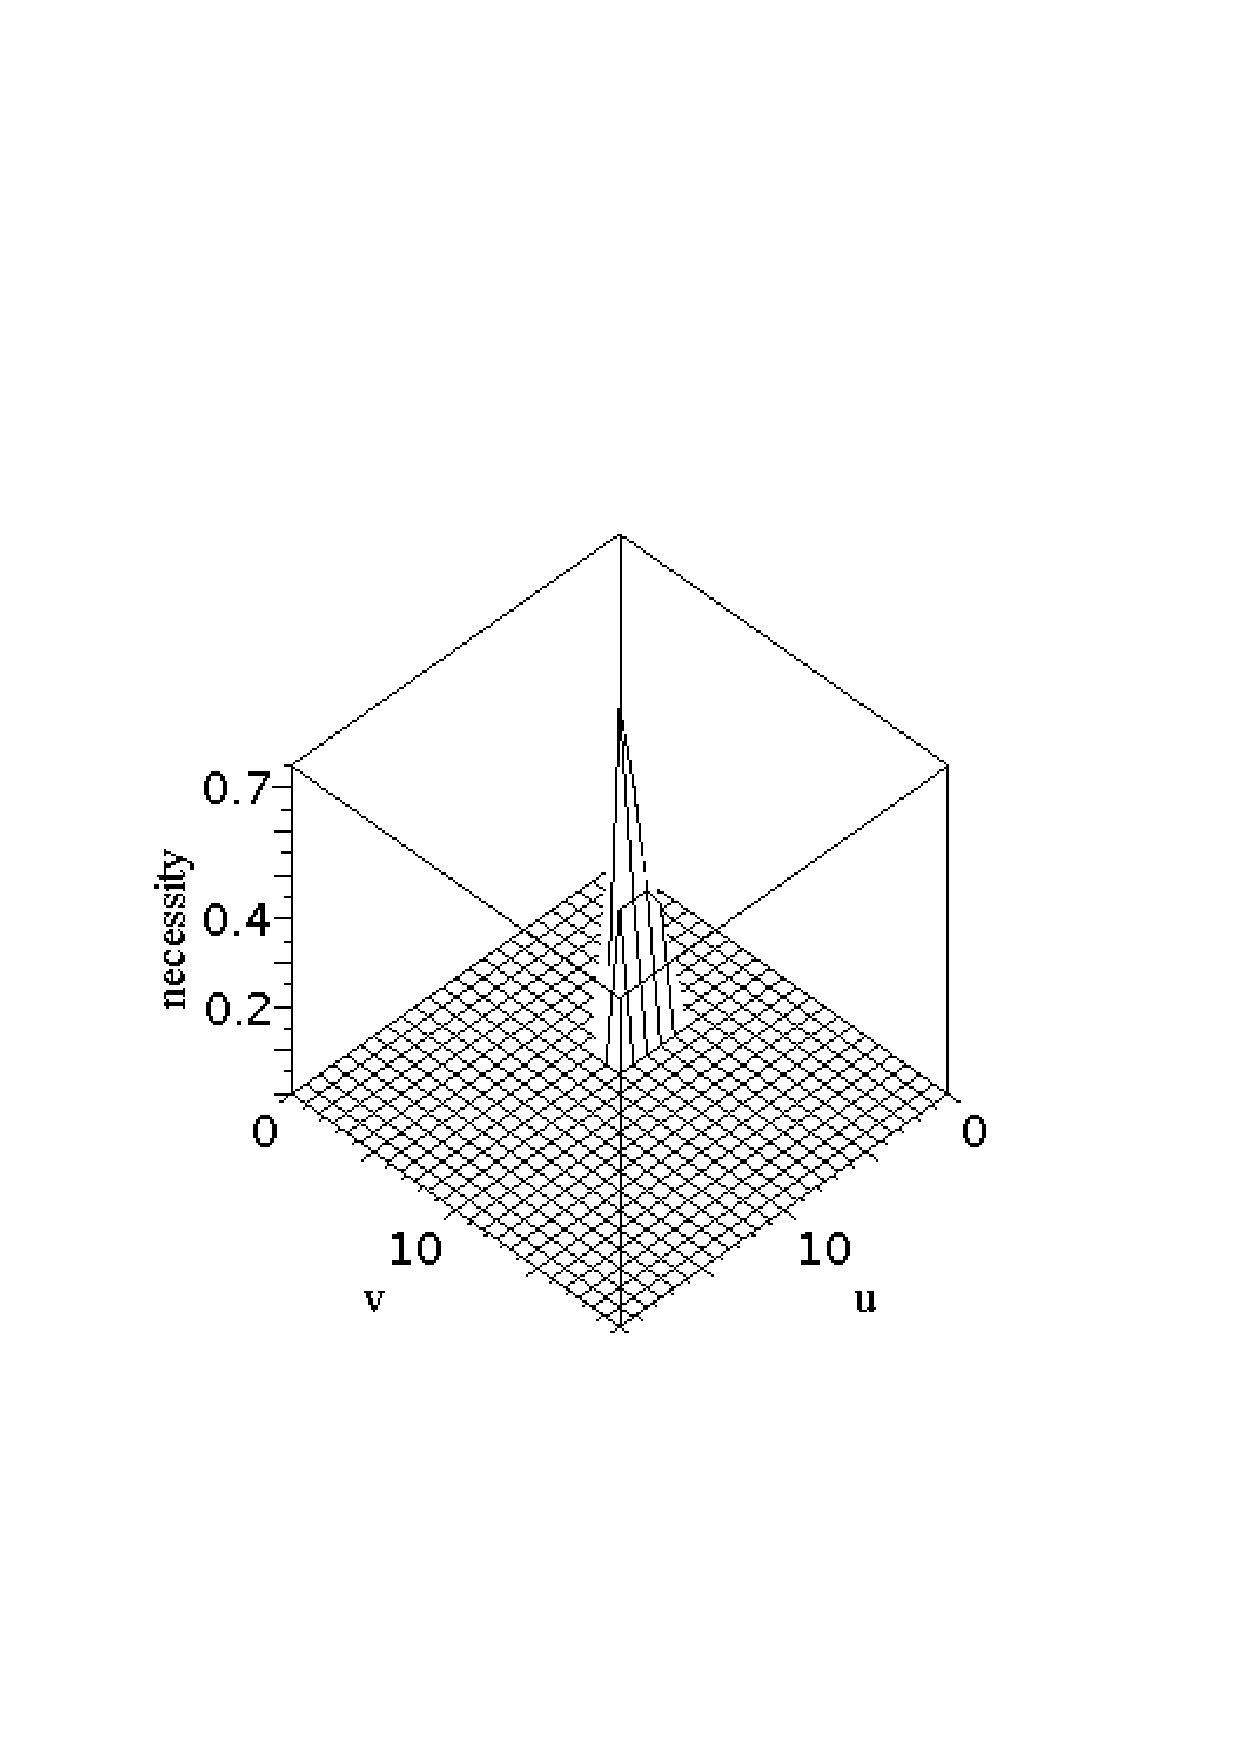
\includegraphics[scale=0.4]{graphs/3D_necessity.pdf}
\caption{Necessity of evaluation for the interval $[a,b]$.}
\label{fig:3d-necessity}
\end{figure}


\section{\label{sec:analysis}ANALYSIS OF PROPOSED TRANSFORMATIONS}

There are several proposals to transform two fuzzy numbers that represent an ill-known interval into one fuzzy interval. This reasoning is however not consistent with possibility theory. We provide several arguments to prove this, which have been previously reasoned by Dubois and Prade \cite{Dubois88b}:

\begin{enumerate}
\item
The fuzzy set given by the two fuzzy numbers is conceptually different from a fuzzy set represented by the fuzzy interval. The fuzzy set given by the two fuzzy numbers belong to $\Pow(\mathbb{R})$ while the fuzzy interval obtained after the transformation is not a possibility distribution on $\Pow(\mathbb{R})$  but on $\mathbb{R}$.
\item
In some cases, (like in the convex hull transformation) because of the underlying ordered domain, the membership function provided for the fuzzy interval preserves the possibility. However, the necessity is not preserved at all.
\end{enumerate}

In the next subsections we will analyze the two major approaches: The transformation that preserves the imprecision and the convex hull. 




\subsection{\label{subsubsec:transf-pres-imp}Transformation that preserves the imprecision}
\begin{figure}[h!]
  \centering
  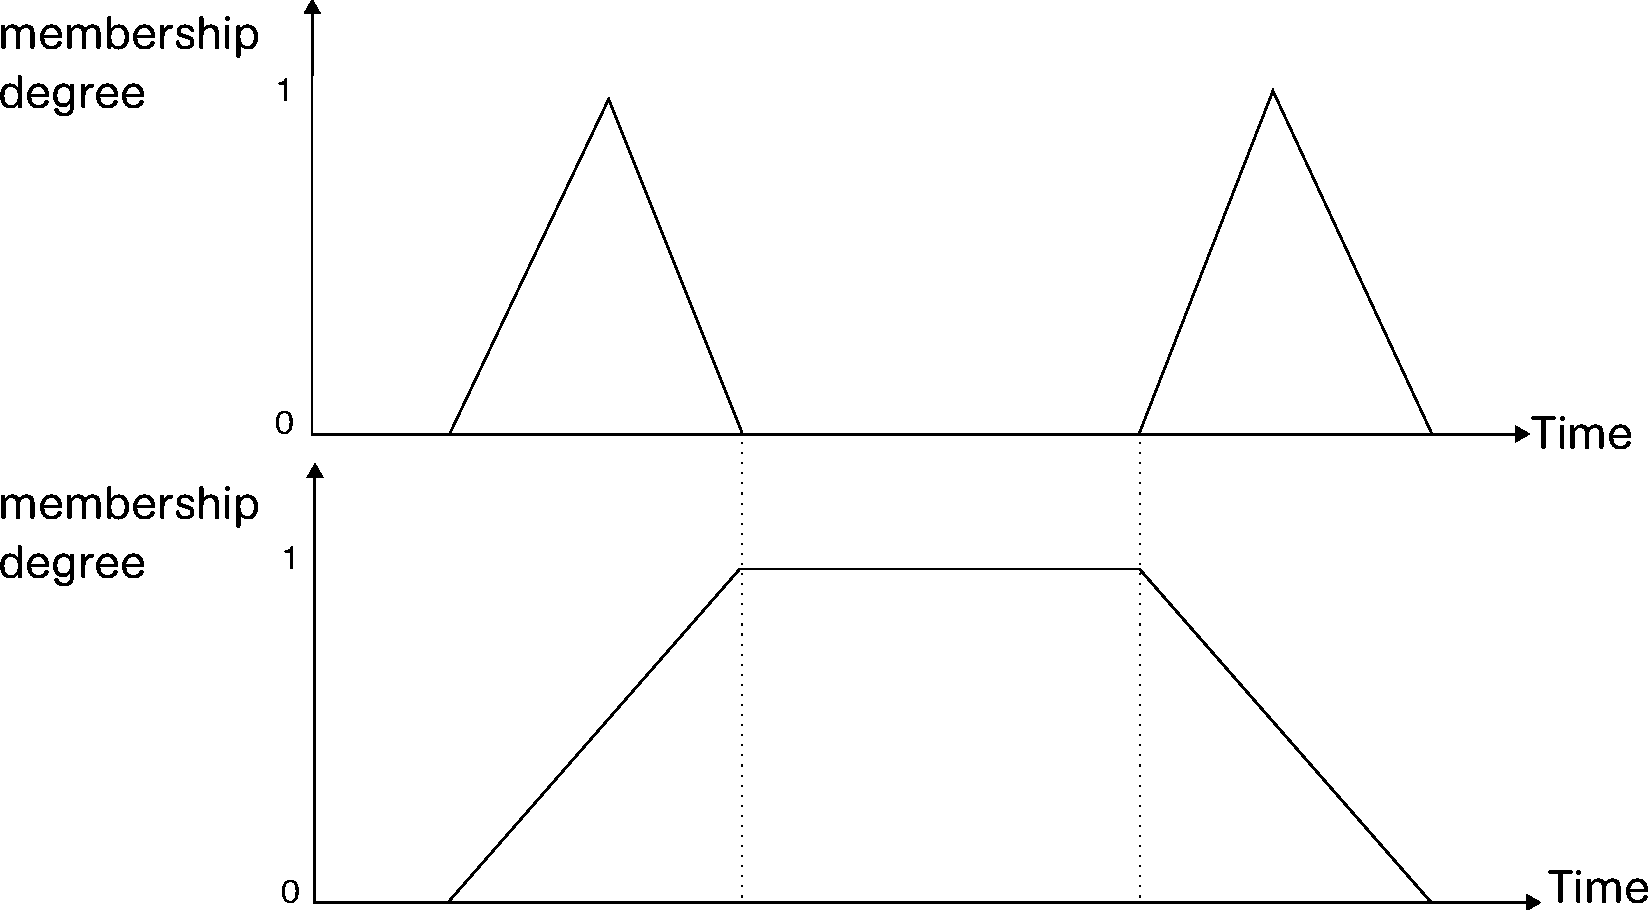
\includegraphics[scale=0.2]{graphs/preservingImprecision.pdf}
  \caption{Transformation of two fuzzy numbers into one fuzzy interval preserving the amount of imprecision.}
  \label{fig:transf-pres-imp}
\end{figure}
This transformation has been proposed in \cite{Garrido2009}. They assume that the imprecision of a fuzzy set is its area. Therefore the transformation consists of preserving the area of both fuzzy numbers that compose the interval. The transformation is performed by means of geometrical computations. The starting point of the fuzzy temporal interval is given by the fuzzy number $S = [d_s,a_s,b_s]$ respectively, the ending point of the fuzzy interval is given by $E = [d_e,a_e,b_e]$ (see Figure \ref{fig:transf-pres-imp}).

The transformation defines a fuzzy interval $T$ by means of a trapezoidal membership function. In order to define the membership function for the fuzzy interval, the following two equalities between the areas from the fuzzy numbers and the fuzzy interval are forced: $S1=S2$ and $S3=S4$. The calculation for the first equality, based on triangle equivalence is:

\begin{equation}
\label{eq:preserving-imprecision}
S1=S2 \Rightarrow \frac{\left(d_s+b_s\right)-\left(d_s-a_s\right)}{2}
\end{equation}        			
The calculation for the right side ($S3=S4$) is analogous.
This transformation is specially widely used when transforming fuzzy time points into fuzzy intervals. The reasoning is the following: the core of the transformed fuzzy interval corresponds with the time when the fact happened. The left and right slopes of the possibility distribution show the imprecision around the starting and the ending times. 

The membership function for this fuzzy interval T is represented by the trapezoid $\left[\alpha,\ \beta,\ \gamma,\ \delta\right]$:

\begin{align}
\nonumber
\alpha & =  d_s - a_s \\
\nonumber
\beta & = d_s + b_s \\
\nonumber
\gamma &= d_e - a_e \\
\nonumber
\delta &= d_e + b_e 
\end{align}

Note that when the supports of the two fuzzy numbers overlap, this transformation makes no sense.

%\paragraph{Comparison}
%In this subsection we will study the knowledge we have about the interval $[u,v]$ w.r.t. the fuzzy interval $T$  which is built preserving the imprecision as explained in Section \ref{subsubsec:transf-pres-imp}. Note that this approach is only valid when the supports of the original fuzzy numbers $X$ and $Y$ are disjoint (see Example \ref{ex:preserving-imprecision} below). Now, the knowledge we have about a number $u$ w.r.t. the transformated fuzzy interval $T$ is:
%\begin{eqnarray}
%\Pos\left(u\in T\right) &=& \mu_{T}\left(u\right) \\
%\Nec\left(u\in T\right) &=& 1 - \mu_{T}\left(u\right).
%\end{eqnarray}
%Therefore, the knowledge about an interval $[u,v]$ w.r.t. $T$ is:
%\begin{eqnarray}
%\nonumber
%\Pos\left([u,v]=T\right) &= \min \left(\Pos\left(u\in T\right),\Pos\left(v\in T\right)\right) &= \min \left(\mu_{T}\left(u\right),\mu_{T}\left(v\right)\right) \\
%\nonumber
%\Nec\left([u,v]=T\right) &= \min \left(\Nec\left(u\in T\right),\Nec\left(v\in T\right)\right) &= \min \left(1 - \mu_{T}\left(\overline{u},1 - \mu_{T}\left(\overline{v}\right)\right)\right)
%\end{eqnarray}


%\begin{example}
%\label{ex:preserving-imprecision}
\paragraph{Example}
In this example we are going to transform the two ill-known points $X= \left[5, 3, 3 \right]$ and $Y= \left[9, 2, 1 \right]$ into one fuzzy interval $T$ using the preserving the imprecision approach. Again, the two fuzzy numbers are represented by means of two triangular possibility distributions:

Then, following the equation presented in \eqref{eq:preserving-imprecision} we obtain the following trapezoidal shape:
\begin{equation}
\mu_{T}\left(x\right) = [d_s-a_s,d_s+b_s,d_e-a_e,d_e+b_e] = [2,8,7,10]
\end{equation}
This construction make no sense when the supports of the fuzzy numbers are disjoint. It is easy to build a rational membership function just by ordering the elements in the representation (e.g. $[2,7,8,10]$) but then, the amount of imprecision is not preserved at all. 
%\end{example}


\subsection{\label{subsubsec:trans-convex-hull}Transformation based on the convex hull}
The transformation based on the convex hull is more intuitive than the previous one. The transformation builds a trapezoidal possibility distribution with the left slope equal to the left slope of the starting fuzzy number (in the graphic, from $d_s-a_s$ to $d_s$) , the core equal to the interval $[d_s,d_e]$ and the right slope equal to the right slope of the ending fuzzy number (from $d_e$ to $d_e+b_e$). The interpretation of this convex hull is the ``most possible'' starting point and the ``most possible'' ending point. Figure \ref{fig:convexHull} shows the resulting transformation.
\begin{figure}[h!]
  \centering
  \includegraphics[scale=0.4]{graphs/convexHull.pdf}
  \caption{Transformation of two fuzzy numbers into one fuzzy interval with the convex hull approach.}
  \label{fig:convexHull}
\end{figure}

In this approach, the trapezoidal membership function ($\left[\alpha,\ \beta,\ \gamma,\ \delta\right]$) is built in a different way:

\begin{align}
\nonumber
\alpha & =  d_s - a_s \\
\nonumber
\beta & = d_s \\
\nonumber
\gamma &= d_e  \\
\nonumber
\delta &= d_e + b_e 
\end{align}
%\paragraph{Comparison}
%Now, we will compare the knowledge we have about the interval $[u,v]$ w.r.t. the fuzzy interval $T$, which is the result of the convex hull transformation between the two fuzzy numbers $X$ and $Y$. The membership degree for the convex hull is given by:

%\begin{align}
%\label{eq:ch-possibility}
%\Pos\left([u,v]=T\right) &= \Pos\left(p^{\left(1\right)}\right) \cap \Pos\left(p^{\left(4\right)}\right) \\ 
%&= \min \left( \sup_{w \leq d}\ \mu_X\left(w\right) , \sup_{w \geq d}\ \mu_Y\left(w\right)\right)
%\end{align}

%The necessity measure for the convex hull is not consistent with the necessity measure for the individual fuzzy numbers $X$ and $Y$. This transformation results in an information lost.

%The necessity measures for the following predicates:

%\begin{align}
%\Nec\left(p^{\left(1\right)}\right) &=  \inf_{w \geq d} 1 - \mu_T\left(w\right) \\
%\Nec\left(p^{\left(4\right)}\right) &=  \inf_{w \leq d} 1 - \mu_T\left(w\right)
%\end{align}

%Therefore the necessity for the interval $[u,v]$ to be inside the fuzzy interval $T$ is:

%\begin{align}
%\label{eq:ch-necessity}
%\Nec\left([u,v]=T\right) &= \min \left(\Nec\left(p^{\left(1\right)}\right), p^{\left(4\right)}\right) \\
%& \min \left(\inf_{w \geq d} 1 - \mu_T\left(w\right),inf_{w \leq d} 1 - \mu_T\left(w\right)\right)
%\end{align}

%\begin{example}
\paragraph{Example}
In this example we are going to build the convex hull for the two ill-known starting and ending points $X= \left[5, 3, 3\right]$ and $Y = \left[9, 2, 1\right]$.


\begin{figure}[h!]
  \centering
 % \includegraphics[scale=0.2]{graphs/convexHull/convexHull.pdf}
 % GNUPLOT: LaTeX picture
\setlength{\unitlength}{0.240900pt}
\ifx\plotpoint\undefined\newsavebox{\plotpoint}\fi
\sbox{\plotpoint}{\rule[-0.200pt]{0.400pt}{0.400pt}}%
\begin{picture}(930,900)(0,0)
\sbox{\plotpoint}{\rule[-0.200pt]{0.400pt}{0.400pt}}%
\put(211.0,82.0){\rule[-0.200pt]{3.613pt}{0.400pt}}
\put(191,82){\makebox(0,0)[r]{ 0}}
\put(865.0,82.0){\rule[-0.200pt]{3.613pt}{0.400pt}}
\put(211.0,145.0){\rule[-0.200pt]{3.613pt}{0.400pt}}
\put(191,145){\makebox(0,0)[r]{ 0.1}}
\put(865.0,145.0){\rule[-0.200pt]{3.613pt}{0.400pt}}
\put(211.0,208.0){\rule[-0.200pt]{3.613pt}{0.400pt}}
\put(191,208){\makebox(0,0)[r]{ 0.2}}
\put(865.0,208.0){\rule[-0.200pt]{3.613pt}{0.400pt}}
\put(211.0,272.0){\rule[-0.200pt]{3.613pt}{0.400pt}}
\put(191,272){\makebox(0,0)[r]{ 0.3}}
\put(865.0,272.0){\rule[-0.200pt]{3.613pt}{0.400pt}}
\put(211.0,335.0){\rule[-0.200pt]{3.613pt}{0.400pt}}
\put(191,335){\makebox(0,0)[r]{ 0.4}}
\put(865.0,335.0){\rule[-0.200pt]{3.613pt}{0.400pt}}
\put(211.0,398.0){\rule[-0.200pt]{3.613pt}{0.400pt}}
\put(191,398){\makebox(0,0)[r]{ 0.5}}
\put(865.0,398.0){\rule[-0.200pt]{3.613pt}{0.400pt}}
\put(211.0,461.0){\rule[-0.200pt]{3.613pt}{0.400pt}}
\put(191,461){\makebox(0,0)[r]{ 0.6}}
\put(865.0,461.0){\rule[-0.200pt]{3.613pt}{0.400pt}}
\put(211.0,524.0){\rule[-0.200pt]{3.613pt}{0.400pt}}
\put(191,524){\makebox(0,0)[r]{ 0.7}}
\put(865.0,524.0){\rule[-0.200pt]{3.613pt}{0.400pt}}
\put(211.0,587.0){\rule[-0.200pt]{3.613pt}{0.400pt}}
\put(191,587){\makebox(0,0)[r]{ 0.8}}
\put(865.0,587.0){\rule[-0.200pt]{3.613pt}{0.400pt}}
\put(211.0,651.0){\rule[-0.200pt]{3.613pt}{0.400pt}}
\put(191,651){\makebox(0,0)[r]{ 0.9}}
\put(865.0,651.0){\rule[-0.200pt]{3.613pt}{0.400pt}}
\put(211.0,714.0){\rule[-0.200pt]{3.613pt}{0.400pt}}
\put(191,714){\makebox(0,0)[r]{ 1}}
\put(865.0,714.0){\rule[-0.200pt]{3.613pt}{0.400pt}}
\put(211.0,777.0){\rule[-0.200pt]{3.613pt}{0.400pt}}
\put(191,777){\makebox(0,0)[r]{ 1.1}}
\put(865.0,777.0){\rule[-0.200pt]{3.613pt}{0.400pt}}
\put(211.0,82.0){\rule[-0.200pt]{0.400pt}{3.613pt}}
\put(211,41){\makebox(0,0){ 0}}
\put(211.0,762.0){\rule[-0.200pt]{0.400pt}{3.613pt}}
\put(278.0,82.0){\rule[-0.200pt]{0.400pt}{3.613pt}}
\put(278,41){\makebox(0,0){ 1}}
\put(278.0,762.0){\rule[-0.200pt]{0.400pt}{3.613pt}}
\put(345.0,82.0){\rule[-0.200pt]{0.400pt}{3.613pt}}
\put(345,41){\makebox(0,0){ 2}}
\put(345.0,762.0){\rule[-0.200pt]{0.400pt}{3.613pt}}
\put(412.0,82.0){\rule[-0.200pt]{0.400pt}{3.613pt}}
\put(412,41){\makebox(0,0){ 3}}
\put(412.0,762.0){\rule[-0.200pt]{0.400pt}{3.613pt}}
\put(479.0,82.0){\rule[-0.200pt]{0.400pt}{3.613pt}}
\put(479,41){\makebox(0,0){ 4}}
\put(479.0,762.0){\rule[-0.200pt]{0.400pt}{3.613pt}}
\put(546.0,82.0){\rule[-0.200pt]{0.400pt}{3.613pt}}
\put(546,41){\makebox(0,0){ 5}}
\put(546.0,762.0){\rule[-0.200pt]{0.400pt}{3.613pt}}
\put(612.0,82.0){\rule[-0.200pt]{0.400pt}{3.613pt}}
\put(612,41){\makebox(0,0){ 6}}
\put(612.0,762.0){\rule[-0.200pt]{0.400pt}{3.613pt}}
\put(679.0,82.0){\rule[-0.200pt]{0.400pt}{3.613pt}}
\put(679,41){\makebox(0,0){ 7}}
\put(679.0,762.0){\rule[-0.200pt]{0.400pt}{3.613pt}}
\put(746.0,82.0){\rule[-0.200pt]{0.400pt}{3.613pt}}
\put(746,41){\makebox(0,0){ 8}}
\put(746.0,762.0){\rule[-0.200pt]{0.400pt}{3.613pt}}
\put(813.0,82.0){\rule[-0.200pt]{0.400pt}{3.613pt}}
\put(813,41){\makebox(0,0){ 9}}
\put(813.0,762.0){\rule[-0.200pt]{0.400pt}{3.613pt}}
\put(880.0,82.0){\rule[-0.200pt]{0.400pt}{3.613pt}}
\put(880,41){\makebox(0,0){ 10}}
\put(880.0,762.0){\rule[-0.200pt]{0.400pt}{3.613pt}}
\put(211.0,82.0){\rule[-0.200pt]{0.400pt}{167.425pt}}
\put(211.0,82.0){\rule[-0.200pt]{161.162pt}{0.400pt}}
\put(880.0,82.0){\rule[-0.200pt]{0.400pt}{167.425pt}}
\put(211.0,777.0){\rule[-0.200pt]{161.162pt}{0.400pt}}
\put(70,429){\makebox(0,0){Possibility}}
\put(545,839){\makebox(0,0){Convex hull Transformation}}
\sbox{\plotpoint}{\rule[-0.400pt]{0.800pt}{0.800pt}}%
\sbox{\plotpoint}{\rule[-0.200pt]{0.400pt}{0.400pt}}%
\put(339,694){\makebox(0,0)[r]{T}}
\sbox{\plotpoint}{\rule[-0.400pt]{0.800pt}{0.800pt}}%
\put(359.0,694.0){\rule[-0.400pt]{24.090pt}{0.800pt}}
\put(211,82){\usebox{\plotpoint}}
\put(339,82.34){\rule{1.600pt}{0.800pt}}
\multiput(339.00,80.34)(3.679,4.000){2}{\rule{0.800pt}{0.800pt}}
\multiput(347.40,86.00)(0.526,1.789){7}{\rule{0.127pt}{2.714pt}}
\multiput(344.34,86.00)(7.000,16.366){2}{\rule{0.800pt}{1.357pt}}
\multiput(354.40,108.00)(0.526,1.701){7}{\rule{0.127pt}{2.600pt}}
\multiput(351.34,108.00)(7.000,15.604){2}{\rule{0.800pt}{1.300pt}}
\multiput(361.39,129.00)(0.536,2.137){5}{\rule{0.129pt}{3.000pt}}
\multiput(358.34,129.00)(6.000,14.773){2}{\rule{0.800pt}{1.500pt}}
\multiput(367.40,150.00)(0.526,1.701){7}{\rule{0.127pt}{2.600pt}}
\multiput(364.34,150.00)(7.000,15.604){2}{\rule{0.800pt}{1.300pt}}
\multiput(374.40,171.00)(0.526,1.789){7}{\rule{0.127pt}{2.714pt}}
\multiput(371.34,171.00)(7.000,16.366){2}{\rule{0.800pt}{1.357pt}}
\multiput(381.40,193.00)(0.526,1.701){7}{\rule{0.127pt}{2.600pt}}
\multiput(378.34,193.00)(7.000,15.604){2}{\rule{0.800pt}{1.300pt}}
\multiput(388.39,214.00)(0.536,2.137){5}{\rule{0.129pt}{3.000pt}}
\multiput(385.34,214.00)(6.000,14.773){2}{\rule{0.800pt}{1.500pt}}
\multiput(394.40,235.00)(0.526,1.701){7}{\rule{0.127pt}{2.600pt}}
\multiput(391.34,235.00)(7.000,15.604){2}{\rule{0.800pt}{1.300pt}}
\multiput(401.40,256.00)(0.526,1.789){7}{\rule{0.127pt}{2.714pt}}
\multiput(398.34,256.00)(7.000,16.366){2}{\rule{0.800pt}{1.357pt}}
\multiput(408.40,278.00)(0.526,1.701){7}{\rule{0.127pt}{2.600pt}}
\multiput(405.34,278.00)(7.000,15.604){2}{\rule{0.800pt}{1.300pt}}
\multiput(415.39,299.00)(0.536,2.137){5}{\rule{0.129pt}{3.000pt}}
\multiput(412.34,299.00)(6.000,14.773){2}{\rule{0.800pt}{1.500pt}}
\multiput(421.40,320.00)(0.526,1.789){7}{\rule{0.127pt}{2.714pt}}
\multiput(418.34,320.00)(7.000,16.366){2}{\rule{0.800pt}{1.357pt}}
\multiput(428.40,342.00)(0.526,1.701){7}{\rule{0.127pt}{2.600pt}}
\multiput(425.34,342.00)(7.000,15.604){2}{\rule{0.800pt}{1.300pt}}
\multiput(435.40,363.00)(0.526,1.701){7}{\rule{0.127pt}{2.600pt}}
\multiput(432.34,363.00)(7.000,15.604){2}{\rule{0.800pt}{1.300pt}}
\multiput(442.40,384.00)(0.526,1.701){7}{\rule{0.127pt}{2.600pt}}
\multiput(439.34,384.00)(7.000,15.604){2}{\rule{0.800pt}{1.300pt}}
\multiput(449.39,405.00)(0.536,2.248){5}{\rule{0.129pt}{3.133pt}}
\multiput(446.34,405.00)(6.000,15.497){2}{\rule{0.800pt}{1.567pt}}
\multiput(455.40,427.00)(0.526,1.701){7}{\rule{0.127pt}{2.600pt}}
\multiput(452.34,427.00)(7.000,15.604){2}{\rule{0.800pt}{1.300pt}}
\multiput(462.40,448.00)(0.526,1.701){7}{\rule{0.127pt}{2.600pt}}
\multiput(459.34,448.00)(7.000,15.604){2}{\rule{0.800pt}{1.300pt}}
\multiput(469.40,469.00)(0.526,1.701){7}{\rule{0.127pt}{2.600pt}}
\multiput(466.34,469.00)(7.000,15.604){2}{\rule{0.800pt}{1.300pt}}
\multiput(476.39,490.00)(0.536,2.248){5}{\rule{0.129pt}{3.133pt}}
\multiput(473.34,490.00)(6.000,15.497){2}{\rule{0.800pt}{1.567pt}}
\multiput(482.40,512.00)(0.526,1.701){7}{\rule{0.127pt}{2.600pt}}
\multiput(479.34,512.00)(7.000,15.604){2}{\rule{0.800pt}{1.300pt}}
\multiput(489.40,533.00)(0.526,1.701){7}{\rule{0.127pt}{2.600pt}}
\multiput(486.34,533.00)(7.000,15.604){2}{\rule{0.800pt}{1.300pt}}
\multiput(496.40,554.00)(0.526,1.789){7}{\rule{0.127pt}{2.714pt}}
\multiput(493.34,554.00)(7.000,16.366){2}{\rule{0.800pt}{1.357pt}}
\multiput(503.39,576.00)(0.536,2.137){5}{\rule{0.129pt}{3.000pt}}
\multiput(500.34,576.00)(6.000,14.773){2}{\rule{0.800pt}{1.500pt}}
\multiput(509.40,597.00)(0.526,1.701){7}{\rule{0.127pt}{2.600pt}}
\multiput(506.34,597.00)(7.000,15.604){2}{\rule{0.800pt}{1.300pt}}
\multiput(516.40,618.00)(0.526,1.701){7}{\rule{0.127pt}{2.600pt}}
\multiput(513.34,618.00)(7.000,15.604){2}{\rule{0.800pt}{1.300pt}}
\multiput(523.40,639.00)(0.526,1.789){7}{\rule{0.127pt}{2.714pt}}
\multiput(520.34,639.00)(7.000,16.366){2}{\rule{0.800pt}{1.357pt}}
\multiput(530.39,661.00)(0.536,2.137){5}{\rule{0.129pt}{3.000pt}}
\multiput(527.34,661.00)(6.000,14.773){2}{\rule{0.800pt}{1.500pt}}
\multiput(536.40,682.00)(0.526,1.701){7}{\rule{0.127pt}{2.600pt}}
\multiput(533.34,682.00)(7.000,15.604){2}{\rule{0.800pt}{1.300pt}}
\multiput(543.40,703.00)(0.526,0.825){7}{\rule{0.127pt}{1.457pt}}
\multiput(540.34,703.00)(7.000,7.976){2}{\rule{0.800pt}{0.729pt}}
\put(211.0,82.0){\rule[-0.400pt]{30.835pt}{0.800pt}}
\multiput(813.40,685.65)(0.526,-4.942){7}{\rule{0.127pt}{6.829pt}}
\multiput(810.34,699.83)(7.000,-43.827){2}{\rule{0.800pt}{3.414pt}}
\multiput(820.40,625.28)(0.526,-5.380){7}{\rule{0.127pt}{7.400pt}}
\multiput(817.34,640.64)(7.000,-47.641){2}{\rule{0.800pt}{3.700pt}}
\multiput(827.40,561.81)(0.526,-5.468){7}{\rule{0.127pt}{7.514pt}}
\multiput(824.34,577.40)(7.000,-48.404){2}{\rule{0.800pt}{3.757pt}}
\multiput(834.39,492.75)(0.536,-6.937){5}{\rule{0.129pt}{8.733pt}}
\multiput(831.34,510.87)(6.000,-45.874){2}{\rule{0.800pt}{4.367pt}}
\multiput(840.40,433.81)(0.526,-5.468){7}{\rule{0.127pt}{7.514pt}}
\multiput(837.34,449.40)(7.000,-48.404){2}{\rule{0.800pt}{3.757pt}}
\multiput(847.40,369.81)(0.526,-5.468){7}{\rule{0.127pt}{7.514pt}}
\multiput(844.34,385.40)(7.000,-48.404){2}{\rule{0.800pt}{3.757pt}}
\multiput(854.40,305.81)(0.526,-5.468){7}{\rule{0.127pt}{7.514pt}}
\multiput(851.34,321.40)(7.000,-48.404){2}{\rule{0.800pt}{3.757pt}}
\multiput(861.39,237.30)(0.536,-6.825){5}{\rule{0.129pt}{8.600pt}}
\multiput(858.34,255.15)(6.000,-45.150){2}{\rule{0.800pt}{4.300pt}}
\multiput(867.40,178.81)(0.526,-5.468){7}{\rule{0.127pt}{7.514pt}}
\multiput(864.34,194.40)(7.000,-48.404){2}{\rule{0.800pt}{3.757pt}}
\multiput(874.40,114.81)(0.526,-5.468){7}{\rule{0.127pt}{7.514pt}}
\multiput(871.34,130.40)(7.000,-48.404){2}{\rule{0.800pt}{3.757pt}}
\put(211,82){\circle{18}}
\put(218,82){\circle{18}}
\put(225,82){\circle{18}}
\put(231,82){\circle{18}}
\put(238,82){\circle{18}}
\put(245,82){\circle{18}}
\put(252,82){\circle{18}}
\put(258,82){\circle{18}}
\put(265,82){\circle{18}}
\put(272,82){\circle{18}}
\put(279,82){\circle{18}}
\put(285,82){\circle{18}}
\put(292,82){\circle{18}}
\put(299,82){\circle{18}}
\put(306,82){\circle{18}}
\put(312,82){\circle{18}}
\put(319,82){\circle{18}}
\put(326,82){\circle{18}}
\put(333,82){\circle{18}}
\put(339,82){\circle{18}}
\put(346,86){\circle{18}}
\put(353,108){\circle{18}}
\put(360,129){\circle{18}}
\put(366,150){\circle{18}}
\put(373,171){\circle{18}}
\put(380,193){\circle{18}}
\put(387,214){\circle{18}}
\put(393,235){\circle{18}}
\put(400,256){\circle{18}}
\put(407,278){\circle{18}}
\put(414,299){\circle{18}}
\put(420,320){\circle{18}}
\put(427,342){\circle{18}}
\put(434,363){\circle{18}}
\put(441,384){\circle{18}}
\put(448,405){\circle{18}}
\put(454,427){\circle{18}}
\put(461,448){\circle{18}}
\put(468,469){\circle{18}}
\put(475,490){\circle{18}}
\put(481,512){\circle{18}}
\put(488,533){\circle{18}}
\put(495,554){\circle{18}}
\put(502,576){\circle{18}}
\put(508,597){\circle{18}}
\put(515,618){\circle{18}}
\put(522,639){\circle{18}}
\put(529,661){\circle{18}}
\put(535,682){\circle{18}}
\put(542,703){\circle{18}}
\put(549,714){\circle{18}}
\put(556,714){\circle{18}}
\put(562,714){\circle{18}}
\put(569,714){\circle{18}}
\put(576,714){\circle{18}}
\put(583,714){\circle{18}}
\put(589,714){\circle{18}}
\put(596,714){\circle{18}}
\put(603,714){\circle{18}}
\put(610,714){\circle{18}}
\put(616,714){\circle{18}}
\put(623,714){\circle{18}}
\put(630,714){\circle{18}}
\put(637,714){\circle{18}}
\put(643,714){\circle{18}}
\put(650,714){\circle{18}}
\put(657,714){\circle{18}}
\put(664,714){\circle{18}}
\put(671,714){\circle{18}}
\put(677,714){\circle{18}}
\put(684,714){\circle{18}}
\put(691,714){\circle{18}}
\put(698,714){\circle{18}}
\put(704,714){\circle{18}}
\put(711,714){\circle{18}}
\put(718,714){\circle{18}}
\put(725,714){\circle{18}}
\put(731,714){\circle{18}}
\put(738,714){\circle{18}}
\put(745,714){\circle{18}}
\put(752,714){\circle{18}}
\put(758,714){\circle{18}}
\put(765,714){\circle{18}}
\put(772,714){\circle{18}}
\put(779,714){\circle{18}}
\put(785,714){\circle{18}}
\put(792,714){\circle{18}}
\put(799,714){\circle{18}}
\put(806,714){\circle{18}}
\put(812,714){\circle{18}}
\put(819,656){\circle{18}}
\put(826,593){\circle{18}}
\put(833,529){\circle{18}}
\put(839,465){\circle{18}}
\put(846,401){\circle{18}}
\put(853,337){\circle{18}}
\put(860,273){\circle{18}}
\put(866,210){\circle{18}}
\put(873,146){\circle{18}}
\put(880,82){\circle{18}}
\put(409,694){\circle{18}}
\put(549.0,714.0){\rule[-0.400pt]{63.357pt}{0.800pt}}
\sbox{\plotpoint}{\rule[-0.200pt]{0.400pt}{0.400pt}}%
\put(339,653){\makebox(0,0)[r]{X}}
\put(359.0,653.0){\rule[-0.200pt]{24.090pt}{0.400pt}}
\put(211,82){\usebox{\plotpoint}}
\multiput(339.00,82.60)(0.920,0.468){5}{\rule{0.800pt}{0.113pt}}
\multiput(339.00,81.17)(5.340,4.000){2}{\rule{0.400pt}{0.400pt}}
\multiput(346.59,86.00)(0.485,1.637){11}{\rule{0.117pt}{1.357pt}}
\multiput(345.17,86.00)(7.000,19.183){2}{\rule{0.400pt}{0.679pt}}
\multiput(353.59,108.00)(0.485,1.560){11}{\rule{0.117pt}{1.300pt}}
\multiput(352.17,108.00)(7.000,18.302){2}{\rule{0.400pt}{0.650pt}}
\multiput(360.59,129.00)(0.482,1.847){9}{\rule{0.116pt}{1.500pt}}
\multiput(359.17,129.00)(6.000,17.887){2}{\rule{0.400pt}{0.750pt}}
\multiput(366.59,150.00)(0.485,1.560){11}{\rule{0.117pt}{1.300pt}}
\multiput(365.17,150.00)(7.000,18.302){2}{\rule{0.400pt}{0.650pt}}
\multiput(373.59,171.00)(0.485,1.637){11}{\rule{0.117pt}{1.357pt}}
\multiput(372.17,171.00)(7.000,19.183){2}{\rule{0.400pt}{0.679pt}}
\multiput(380.59,193.00)(0.485,1.560){11}{\rule{0.117pt}{1.300pt}}
\multiput(379.17,193.00)(7.000,18.302){2}{\rule{0.400pt}{0.650pt}}
\multiput(387.59,214.00)(0.482,1.847){9}{\rule{0.116pt}{1.500pt}}
\multiput(386.17,214.00)(6.000,17.887){2}{\rule{0.400pt}{0.750pt}}
\multiput(393.59,235.00)(0.485,1.560){11}{\rule{0.117pt}{1.300pt}}
\multiput(392.17,235.00)(7.000,18.302){2}{\rule{0.400pt}{0.650pt}}
\multiput(400.59,256.00)(0.485,1.637){11}{\rule{0.117pt}{1.357pt}}
\multiput(399.17,256.00)(7.000,19.183){2}{\rule{0.400pt}{0.679pt}}
\multiput(407.59,278.00)(0.485,1.560){11}{\rule{0.117pt}{1.300pt}}
\multiput(406.17,278.00)(7.000,18.302){2}{\rule{0.400pt}{0.650pt}}
\multiput(414.59,299.00)(0.482,1.847){9}{\rule{0.116pt}{1.500pt}}
\multiput(413.17,299.00)(6.000,17.887){2}{\rule{0.400pt}{0.750pt}}
\multiput(420.59,320.00)(0.485,1.637){11}{\rule{0.117pt}{1.357pt}}
\multiput(419.17,320.00)(7.000,19.183){2}{\rule{0.400pt}{0.679pt}}
\multiput(427.59,342.00)(0.485,1.560){11}{\rule{0.117pt}{1.300pt}}
\multiput(426.17,342.00)(7.000,18.302){2}{\rule{0.400pt}{0.650pt}}
\multiput(434.59,363.00)(0.485,1.560){11}{\rule{0.117pt}{1.300pt}}
\multiput(433.17,363.00)(7.000,18.302){2}{\rule{0.400pt}{0.650pt}}
\multiput(441.59,384.00)(0.485,1.560){11}{\rule{0.117pt}{1.300pt}}
\multiput(440.17,384.00)(7.000,18.302){2}{\rule{0.400pt}{0.650pt}}
\multiput(448.59,405.00)(0.482,1.937){9}{\rule{0.116pt}{1.567pt}}
\multiput(447.17,405.00)(6.000,18.748){2}{\rule{0.400pt}{0.783pt}}
\multiput(454.59,427.00)(0.485,1.560){11}{\rule{0.117pt}{1.300pt}}
\multiput(453.17,427.00)(7.000,18.302){2}{\rule{0.400pt}{0.650pt}}
\multiput(461.59,448.00)(0.485,1.560){11}{\rule{0.117pt}{1.300pt}}
\multiput(460.17,448.00)(7.000,18.302){2}{\rule{0.400pt}{0.650pt}}
\multiput(468.59,469.00)(0.485,1.560){11}{\rule{0.117pt}{1.300pt}}
\multiput(467.17,469.00)(7.000,18.302){2}{\rule{0.400pt}{0.650pt}}
\multiput(475.59,490.00)(0.482,1.937){9}{\rule{0.116pt}{1.567pt}}
\multiput(474.17,490.00)(6.000,18.748){2}{\rule{0.400pt}{0.783pt}}
\multiput(481.59,512.00)(0.485,1.560){11}{\rule{0.117pt}{1.300pt}}
\multiput(480.17,512.00)(7.000,18.302){2}{\rule{0.400pt}{0.650pt}}
\multiput(488.59,533.00)(0.485,1.560){11}{\rule{0.117pt}{1.300pt}}
\multiput(487.17,533.00)(7.000,18.302){2}{\rule{0.400pt}{0.650pt}}
\multiput(495.59,554.00)(0.485,1.637){11}{\rule{0.117pt}{1.357pt}}
\multiput(494.17,554.00)(7.000,19.183){2}{\rule{0.400pt}{0.679pt}}
\multiput(502.59,576.00)(0.482,1.847){9}{\rule{0.116pt}{1.500pt}}
\multiput(501.17,576.00)(6.000,17.887){2}{\rule{0.400pt}{0.750pt}}
\multiput(508.59,597.00)(0.485,1.560){11}{\rule{0.117pt}{1.300pt}}
\multiput(507.17,597.00)(7.000,18.302){2}{\rule{0.400pt}{0.650pt}}
\multiput(515.59,618.00)(0.485,1.560){11}{\rule{0.117pt}{1.300pt}}
\multiput(514.17,618.00)(7.000,18.302){2}{\rule{0.400pt}{0.650pt}}
\multiput(522.59,639.00)(0.485,1.637){11}{\rule{0.117pt}{1.357pt}}
\multiput(521.17,639.00)(7.000,19.183){2}{\rule{0.400pt}{0.679pt}}
\multiput(529.59,661.00)(0.482,1.847){9}{\rule{0.116pt}{1.500pt}}
\multiput(528.17,661.00)(6.000,17.887){2}{\rule{0.400pt}{0.750pt}}
\multiput(535.59,682.00)(0.485,1.560){11}{\rule{0.117pt}{1.300pt}}
\multiput(534.17,682.00)(7.000,18.302){2}{\rule{0.400pt}{0.650pt}}
\put(211.0,82.0){\rule[-0.200pt]{30.835pt}{0.400pt}}
\multiput(549.59,697.60)(0.485,-1.560){11}{\rule{0.117pt}{1.300pt}}
\multiput(548.17,700.30)(7.000,-18.302){2}{\rule{0.400pt}{0.650pt}}
\multiput(556.59,675.77)(0.482,-1.847){9}{\rule{0.116pt}{1.500pt}}
\multiput(555.17,678.89)(6.000,-17.887){2}{\rule{0.400pt}{0.750pt}}
\multiput(562.59,655.37)(0.485,-1.637){11}{\rule{0.117pt}{1.357pt}}
\multiput(561.17,658.18)(7.000,-19.183){2}{\rule{0.400pt}{0.679pt}}
\multiput(569.59,633.60)(0.485,-1.560){11}{\rule{0.117pt}{1.300pt}}
\multiput(568.17,636.30)(7.000,-18.302){2}{\rule{0.400pt}{0.650pt}}
\multiput(576.59,612.60)(0.485,-1.560){11}{\rule{0.117pt}{1.300pt}}
\multiput(575.17,615.30)(7.000,-18.302){2}{\rule{0.400pt}{0.650pt}}
\multiput(583.59,590.77)(0.482,-1.847){9}{\rule{0.116pt}{1.500pt}}
\multiput(582.17,593.89)(6.000,-17.887){2}{\rule{0.400pt}{0.750pt}}
\multiput(589.59,570.37)(0.485,-1.637){11}{\rule{0.117pt}{1.357pt}}
\multiput(588.17,573.18)(7.000,-19.183){2}{\rule{0.400pt}{0.679pt}}
\multiput(596.59,548.60)(0.485,-1.560){11}{\rule{0.117pt}{1.300pt}}
\multiput(595.17,551.30)(7.000,-18.302){2}{\rule{0.400pt}{0.650pt}}
\multiput(603.59,527.60)(0.485,-1.560){11}{\rule{0.117pt}{1.300pt}}
\multiput(602.17,530.30)(7.000,-18.302){2}{\rule{0.400pt}{0.650pt}}
\multiput(610.59,505.50)(0.482,-1.937){9}{\rule{0.116pt}{1.567pt}}
\multiput(609.17,508.75)(6.000,-18.748){2}{\rule{0.400pt}{0.783pt}}
\multiput(616.59,484.60)(0.485,-1.560){11}{\rule{0.117pt}{1.300pt}}
\multiput(615.17,487.30)(7.000,-18.302){2}{\rule{0.400pt}{0.650pt}}
\multiput(623.59,463.60)(0.485,-1.560){11}{\rule{0.117pt}{1.300pt}}
\multiput(622.17,466.30)(7.000,-18.302){2}{\rule{0.400pt}{0.650pt}}
\multiput(630.59,442.60)(0.485,-1.560){11}{\rule{0.117pt}{1.300pt}}
\multiput(629.17,445.30)(7.000,-18.302){2}{\rule{0.400pt}{0.650pt}}
\multiput(637.59,420.50)(0.482,-1.937){9}{\rule{0.116pt}{1.567pt}}
\multiput(636.17,423.75)(6.000,-18.748){2}{\rule{0.400pt}{0.783pt}}
\multiput(643.59,399.60)(0.485,-1.560){11}{\rule{0.117pt}{1.300pt}}
\multiput(642.17,402.30)(7.000,-18.302){2}{\rule{0.400pt}{0.650pt}}
\multiput(650.59,378.60)(0.485,-1.560){11}{\rule{0.117pt}{1.300pt}}
\multiput(649.17,381.30)(7.000,-18.302){2}{\rule{0.400pt}{0.650pt}}
\multiput(657.59,357.60)(0.485,-1.560){11}{\rule{0.117pt}{1.300pt}}
\multiput(656.17,360.30)(7.000,-18.302){2}{\rule{0.400pt}{0.650pt}}
\multiput(664.59,336.37)(0.485,-1.637){11}{\rule{0.117pt}{1.357pt}}
\multiput(663.17,339.18)(7.000,-19.183){2}{\rule{0.400pt}{0.679pt}}
\multiput(671.59,313.77)(0.482,-1.847){9}{\rule{0.116pt}{1.500pt}}
\multiput(670.17,316.89)(6.000,-17.887){2}{\rule{0.400pt}{0.750pt}}
\multiput(677.59,293.60)(0.485,-1.560){11}{\rule{0.117pt}{1.300pt}}
\multiput(676.17,296.30)(7.000,-18.302){2}{\rule{0.400pt}{0.650pt}}
\multiput(684.59,272.37)(0.485,-1.637){11}{\rule{0.117pt}{1.357pt}}
\multiput(683.17,275.18)(7.000,-19.183){2}{\rule{0.400pt}{0.679pt}}
\multiput(691.59,250.60)(0.485,-1.560){11}{\rule{0.117pt}{1.300pt}}
\multiput(690.17,253.30)(7.000,-18.302){2}{\rule{0.400pt}{0.650pt}}
\multiput(698.59,228.77)(0.482,-1.847){9}{\rule{0.116pt}{1.500pt}}
\multiput(697.17,231.89)(6.000,-17.887){2}{\rule{0.400pt}{0.750pt}}
\multiput(704.59,208.60)(0.485,-1.560){11}{\rule{0.117pt}{1.300pt}}
\multiput(703.17,211.30)(7.000,-18.302){2}{\rule{0.400pt}{0.650pt}}
\multiput(711.59,187.37)(0.485,-1.637){11}{\rule{0.117pt}{1.357pt}}
\multiput(710.17,190.18)(7.000,-19.183){2}{\rule{0.400pt}{0.679pt}}
\multiput(718.59,165.60)(0.485,-1.560){11}{\rule{0.117pt}{1.300pt}}
\multiput(717.17,168.30)(7.000,-18.302){2}{\rule{0.400pt}{0.650pt}}
\multiput(725.59,143.77)(0.482,-1.847){9}{\rule{0.116pt}{1.500pt}}
\multiput(724.17,146.89)(6.000,-17.887){2}{\rule{0.400pt}{0.750pt}}
\multiput(731.59,123.60)(0.485,-1.560){11}{\rule{0.117pt}{1.300pt}}
\multiput(730.17,126.30)(7.000,-18.302){2}{\rule{0.400pt}{0.650pt}}
\multiput(738.59,102.37)(0.485,-1.637){11}{\rule{0.117pt}{1.357pt}}
\multiput(737.17,105.18)(7.000,-19.183){2}{\rule{0.400pt}{0.679pt}}
\multiput(745.00,84.94)(0.920,-0.468){5}{\rule{0.800pt}{0.113pt}}
\multiput(745.00,85.17)(5.340,-4.000){2}{\rule{0.400pt}{0.400pt}}
\put(542.0,703.0){\rule[-0.200pt]{1.686pt}{0.400pt}}
\put(211,82){\makebox(0,0){$\times$}}
\put(218,82){\makebox(0,0){$\times$}}
\put(225,82){\makebox(0,0){$\times$}}
\put(231,82){\makebox(0,0){$\times$}}
\put(238,82){\makebox(0,0){$\times$}}
\put(245,82){\makebox(0,0){$\times$}}
\put(252,82){\makebox(0,0){$\times$}}
\put(258,82){\makebox(0,0){$\times$}}
\put(265,82){\makebox(0,0){$\times$}}
\put(272,82){\makebox(0,0){$\times$}}
\put(279,82){\makebox(0,0){$\times$}}
\put(285,82){\makebox(0,0){$\times$}}
\put(292,82){\makebox(0,0){$\times$}}
\put(299,82){\makebox(0,0){$\times$}}
\put(306,82){\makebox(0,0){$\times$}}
\put(312,82){\makebox(0,0){$\times$}}
\put(319,82){\makebox(0,0){$\times$}}
\put(326,82){\makebox(0,0){$\times$}}
\put(333,82){\makebox(0,0){$\times$}}
\put(339,82){\makebox(0,0){$\times$}}
\put(346,86){\makebox(0,0){$\times$}}
\put(353,108){\makebox(0,0){$\times$}}
\put(360,129){\makebox(0,0){$\times$}}
\put(366,150){\makebox(0,0){$\times$}}
\put(373,171){\makebox(0,0){$\times$}}
\put(380,193){\makebox(0,0){$\times$}}
\put(387,214){\makebox(0,0){$\times$}}
\put(393,235){\makebox(0,0){$\times$}}
\put(400,256){\makebox(0,0){$\times$}}
\put(407,278){\makebox(0,0){$\times$}}
\put(414,299){\makebox(0,0){$\times$}}
\put(420,320){\makebox(0,0){$\times$}}
\put(427,342){\makebox(0,0){$\times$}}
\put(434,363){\makebox(0,0){$\times$}}
\put(441,384){\makebox(0,0){$\times$}}
\put(448,405){\makebox(0,0){$\times$}}
\put(454,427){\makebox(0,0){$\times$}}
\put(461,448){\makebox(0,0){$\times$}}
\put(468,469){\makebox(0,0){$\times$}}
\put(475,490){\makebox(0,0){$\times$}}
\put(481,512){\makebox(0,0){$\times$}}
\put(488,533){\makebox(0,0){$\times$}}
\put(495,554){\makebox(0,0){$\times$}}
\put(502,576){\makebox(0,0){$\times$}}
\put(508,597){\makebox(0,0){$\times$}}
\put(515,618){\makebox(0,0){$\times$}}
\put(522,639){\makebox(0,0){$\times$}}
\put(529,661){\makebox(0,0){$\times$}}
\put(535,682){\makebox(0,0){$\times$}}
\put(542,703){\makebox(0,0){$\times$}}
\put(549,703){\makebox(0,0){$\times$}}
\put(556,682){\makebox(0,0){$\times$}}
\put(562,661){\makebox(0,0){$\times$}}
\put(569,639){\makebox(0,0){$\times$}}
\put(576,618){\makebox(0,0){$\times$}}
\put(583,597){\makebox(0,0){$\times$}}
\put(589,576){\makebox(0,0){$\times$}}
\put(596,554){\makebox(0,0){$\times$}}
\put(603,533){\makebox(0,0){$\times$}}
\put(610,512){\makebox(0,0){$\times$}}
\put(616,490){\makebox(0,0){$\times$}}
\put(623,469){\makebox(0,0){$\times$}}
\put(630,448){\makebox(0,0){$\times$}}
\put(637,427){\makebox(0,0){$\times$}}
\put(643,405){\makebox(0,0){$\times$}}
\put(650,384){\makebox(0,0){$\times$}}
\put(657,363){\makebox(0,0){$\times$}}
\put(664,342){\makebox(0,0){$\times$}}
\put(671,320){\makebox(0,0){$\times$}}
\put(677,299){\makebox(0,0){$\times$}}
\put(684,278){\makebox(0,0){$\times$}}
\put(691,256){\makebox(0,0){$\times$}}
\put(698,235){\makebox(0,0){$\times$}}
\put(704,214){\makebox(0,0){$\times$}}
\put(711,193){\makebox(0,0){$\times$}}
\put(718,171){\makebox(0,0){$\times$}}
\put(725,150){\makebox(0,0){$\times$}}
\put(731,129){\makebox(0,0){$\times$}}
\put(738,108){\makebox(0,0){$\times$}}
\put(745,86){\makebox(0,0){$\times$}}
\put(752,82){\makebox(0,0){$\times$}}
\put(758,82){\makebox(0,0){$\times$}}
\put(765,82){\makebox(0,0){$\times$}}
\put(772,82){\makebox(0,0){$\times$}}
\put(779,82){\makebox(0,0){$\times$}}
\put(785,82){\makebox(0,0){$\times$}}
\put(792,82){\makebox(0,0){$\times$}}
\put(799,82){\makebox(0,0){$\times$}}
\put(806,82){\makebox(0,0){$\times$}}
\put(812,82){\makebox(0,0){$\times$}}
\put(819,82){\makebox(0,0){$\times$}}
\put(826,82){\makebox(0,0){$\times$}}
\put(833,82){\makebox(0,0){$\times$}}
\put(839,82){\makebox(0,0){$\times$}}
\put(846,82){\makebox(0,0){$\times$}}
\put(853,82){\makebox(0,0){$\times$}}
\put(860,82){\makebox(0,0){$\times$}}
\put(866,82){\makebox(0,0){$\times$}}
\put(873,82){\makebox(0,0){$\times$}}
\put(880,82){\makebox(0,0){$\times$}}
\put(409,653){\makebox(0,0){$\times$}}
\put(752.0,82.0){\rule[-0.200pt]{30.835pt}{0.400pt}}
\put(339,612){\makebox(0,0)[r]{Y}}
\multiput(359,612)(20.756,0.000){5}{\usebox{\plotpoint}}
\put(459,612){\usebox{\plotpoint}}
\put(211,82){\usebox{\plotpoint}}
\put(211.00,82.00){\usebox{\plotpoint}}
\put(231.76,82.00){\usebox{\plotpoint}}
\put(252.51,82.00){\usebox{\plotpoint}}
\put(273.27,82.00){\usebox{\plotpoint}}
\put(294.02,82.00){\usebox{\plotpoint}}
\put(314.78,82.00){\usebox{\plotpoint}}
\put(335.53,82.00){\usebox{\plotpoint}}
\put(356.29,82.00){\usebox{\plotpoint}}
\put(377.04,82.00){\usebox{\plotpoint}}
\put(397.80,82.00){\usebox{\plotpoint}}
\put(418.55,82.00){\usebox{\plotpoint}}
\put(439.31,82.00){\usebox{\plotpoint}}
\put(460.07,82.00){\usebox{\plotpoint}}
\put(480.82,82.00){\usebox{\plotpoint}}
\put(501.58,82.00){\usebox{\plotpoint}}
\put(522.33,82.00){\usebox{\plotpoint}}
\put(543.09,82.00){\usebox{\plotpoint}}
\put(563.84,82.00){\usebox{\plotpoint}}
\put(584.60,82.00){\usebox{\plotpoint}}
\put(605.35,82.00){\usebox{\plotpoint}}
\put(626.11,82.00){\usebox{\plotpoint}}
\put(646.87,82.00){\usebox{\plotpoint}}
\put(667.62,82.00){\usebox{\plotpoint}}
\put(680.45,92.84){\usebox{\plotpoint}}
\multiput(684,104)(4.435,20.276){2}{\usebox{\plotpoint}}
\put(694.80,153.39){\usebox{\plotpoint}}
\multiput(698,168)(3.825,20.400){2}{\usebox{\plotpoint}}
\put(707.15,214.41){\usebox{\plotpoint}}
\multiput(711,232)(4.435,20.276){2}{\usebox{\plotpoint}}
\multiput(718,264)(4.435,20.276){2}{\usebox{\plotpoint}}
\put(728.73,315.91){\usebox{\plotpoint}}
\multiput(731,328)(4.435,20.276){2}{\usebox{\plotpoint}}
\put(741.68,376.81){\usebox{\plotpoint}}
\multiput(745,392)(4.572,20.246){2}{\usebox{\plotpoint}}
\put(754.75,437.68){\usebox{\plotpoint}}
\multiput(758,455)(4.435,20.276){2}{\usebox{\plotpoint}}
\multiput(765,487)(4.435,20.276){2}{\usebox{\plotpoint}}
\put(776.41,539.17){\usebox{\plotpoint}}
\multiput(779,551)(3.825,20.400){2}{\usebox{\plotpoint}}
\put(788.76,600.19){\usebox{\plotpoint}}
\multiput(792,615)(4.435,20.276){2}{\usebox{\plotpoint}}
\put(802.07,661.02){\usebox{\plotpoint}}
\multiput(806,679)(3.825,20.400){2}{\usebox{\plotpoint}}
\multiput(812,711)(2.620,-20.589){3}{\usebox{\plotpoint}}
\multiput(819,656)(2.292,-20.629){3}{\usebox{\plotpoint}}
\multiput(826,593)(2.257,-20.632){3}{\usebox{\plotpoint}}
\multiput(833,529)(1.937,-20.665){3}{\usebox{\plotpoint}}
\multiput(839,465)(2.257,-20.632){3}{\usebox{\plotpoint}}
\multiput(846,401)(2.257,-20.632){3}{\usebox{\plotpoint}}
\multiput(853,337)(2.257,-20.632){3}{\usebox{\plotpoint}}
\multiput(860,273)(1.968,-20.662){3}{\usebox{\plotpoint}}
\multiput(866,210)(2.257,-20.632){3}{\usebox{\plotpoint}}
\multiput(873,146)(2.257,-20.632){3}{\usebox{\plotpoint}}
\put(880,82){\usebox{\plotpoint}}
\put(211,82){\makebox(0,0){$\star$}}
\put(218,82){\makebox(0,0){$\star$}}
\put(225,82){\makebox(0,0){$\star$}}
\put(231,82){\makebox(0,0){$\star$}}
\put(238,82){\makebox(0,0){$\star$}}
\put(245,82){\makebox(0,0){$\star$}}
\put(252,82){\makebox(0,0){$\star$}}
\put(258,82){\makebox(0,0){$\star$}}
\put(265,82){\makebox(0,0){$\star$}}
\put(272,82){\makebox(0,0){$\star$}}
\put(279,82){\makebox(0,0){$\star$}}
\put(285,82){\makebox(0,0){$\star$}}
\put(292,82){\makebox(0,0){$\star$}}
\put(299,82){\makebox(0,0){$\star$}}
\put(306,82){\makebox(0,0){$\star$}}
\put(312,82){\makebox(0,0){$\star$}}
\put(319,82){\makebox(0,0){$\star$}}
\put(326,82){\makebox(0,0){$\star$}}
\put(333,82){\makebox(0,0){$\star$}}
\put(339,82){\makebox(0,0){$\star$}}
\put(346,82){\makebox(0,0){$\star$}}
\put(353,82){\makebox(0,0){$\star$}}
\put(360,82){\makebox(0,0){$\star$}}
\put(366,82){\makebox(0,0){$\star$}}
\put(373,82){\makebox(0,0){$\star$}}
\put(380,82){\makebox(0,0){$\star$}}
\put(387,82){\makebox(0,0){$\star$}}
\put(393,82){\makebox(0,0){$\star$}}
\put(400,82){\makebox(0,0){$\star$}}
\put(407,82){\makebox(0,0){$\star$}}
\put(414,82){\makebox(0,0){$\star$}}
\put(420,82){\makebox(0,0){$\star$}}
\put(427,82){\makebox(0,0){$\star$}}
\put(434,82){\makebox(0,0){$\star$}}
\put(441,82){\makebox(0,0){$\star$}}
\put(448,82){\makebox(0,0){$\star$}}
\put(454,82){\makebox(0,0){$\star$}}
\put(461,82){\makebox(0,0){$\star$}}
\put(468,82){\makebox(0,0){$\star$}}
\put(475,82){\makebox(0,0){$\star$}}
\put(481,82){\makebox(0,0){$\star$}}
\put(488,82){\makebox(0,0){$\star$}}
\put(495,82){\makebox(0,0){$\star$}}
\put(502,82){\makebox(0,0){$\star$}}
\put(508,82){\makebox(0,0){$\star$}}
\put(515,82){\makebox(0,0){$\star$}}
\put(522,82){\makebox(0,0){$\star$}}
\put(529,82){\makebox(0,0){$\star$}}
\put(535,82){\makebox(0,0){$\star$}}
\put(542,82){\makebox(0,0){$\star$}}
\put(549,82){\makebox(0,0){$\star$}}
\put(556,82){\makebox(0,0){$\star$}}
\put(562,82){\makebox(0,0){$\star$}}
\put(569,82){\makebox(0,0){$\star$}}
\put(576,82){\makebox(0,0){$\star$}}
\put(583,82){\makebox(0,0){$\star$}}
\put(589,82){\makebox(0,0){$\star$}}
\put(596,82){\makebox(0,0){$\star$}}
\put(603,82){\makebox(0,0){$\star$}}
\put(610,82){\makebox(0,0){$\star$}}
\put(616,82){\makebox(0,0){$\star$}}
\put(623,82){\makebox(0,0){$\star$}}
\put(630,82){\makebox(0,0){$\star$}}
\put(637,82){\makebox(0,0){$\star$}}
\put(643,82){\makebox(0,0){$\star$}}
\put(650,82){\makebox(0,0){$\star$}}
\put(657,82){\makebox(0,0){$\star$}}
\put(664,82){\makebox(0,0){$\star$}}
\put(671,82){\makebox(0,0){$\star$}}
\put(677,82){\makebox(0,0){$\star$}}
\put(684,104){\makebox(0,0){$\star$}}
\put(691,136){\makebox(0,0){$\star$}}
\put(698,168){\makebox(0,0){$\star$}}
\put(704,200){\makebox(0,0){$\star$}}
\put(711,232){\makebox(0,0){$\star$}}
\put(718,264){\makebox(0,0){$\star$}}
\put(725,296){\makebox(0,0){$\star$}}
\put(731,328){\makebox(0,0){$\star$}}
\put(738,360){\makebox(0,0){$\star$}}
\put(745,392){\makebox(0,0){$\star$}}
\put(752,423){\makebox(0,0){$\star$}}
\put(758,455){\makebox(0,0){$\star$}}
\put(765,487){\makebox(0,0){$\star$}}
\put(772,519){\makebox(0,0){$\star$}}
\put(779,551){\makebox(0,0){$\star$}}
\put(785,583){\makebox(0,0){$\star$}}
\put(792,615){\makebox(0,0){$\star$}}
\put(799,647){\makebox(0,0){$\star$}}
\put(806,679){\makebox(0,0){$\star$}}
\put(812,711){\makebox(0,0){$\star$}}
\put(819,656){\makebox(0,0){$\star$}}
\put(826,593){\makebox(0,0){$\star$}}
\put(833,529){\makebox(0,0){$\star$}}
\put(839,465){\makebox(0,0){$\star$}}
\put(846,401){\makebox(0,0){$\star$}}
\put(853,337){\makebox(0,0){$\star$}}
\put(860,273){\makebox(0,0){$\star$}}
\put(866,210){\makebox(0,0){$\star$}}
\put(873,146){\makebox(0,0){$\star$}}
\put(880,82){\makebox(0,0){$\star$}}
\put(409,612){\makebox(0,0){$\star$}}
\put(211.0,82.0){\rule[-0.200pt]{0.400pt}{167.425pt}}
\put(211.0,82.0){\rule[-0.200pt]{161.162pt}{0.400pt}}
\put(880.0,82.0){\rule[-0.200pt]{0.400pt}{167.425pt}}
\put(211.0,777.0){\rule[-0.200pt]{161.162pt}{0.400pt}}
\end{picture}

  \caption{Construction of the convex hull $T$ w.r.t the ill-known values $X$ and $Y$.}
  \label{fig:convex-hull-T}
\end{figure}


The convex hull for the fuzzy numbers $X$ and $Y$, represented by means of two triangular possibility distributions results in a trapezoidal possibility distribution with membership function $\mu_T(x)$ (see Figure \ref{fig:convex-hull-T}), represented by $[2,5,9,10]$.

%\begin{figure}[h!]
%  \centering
%  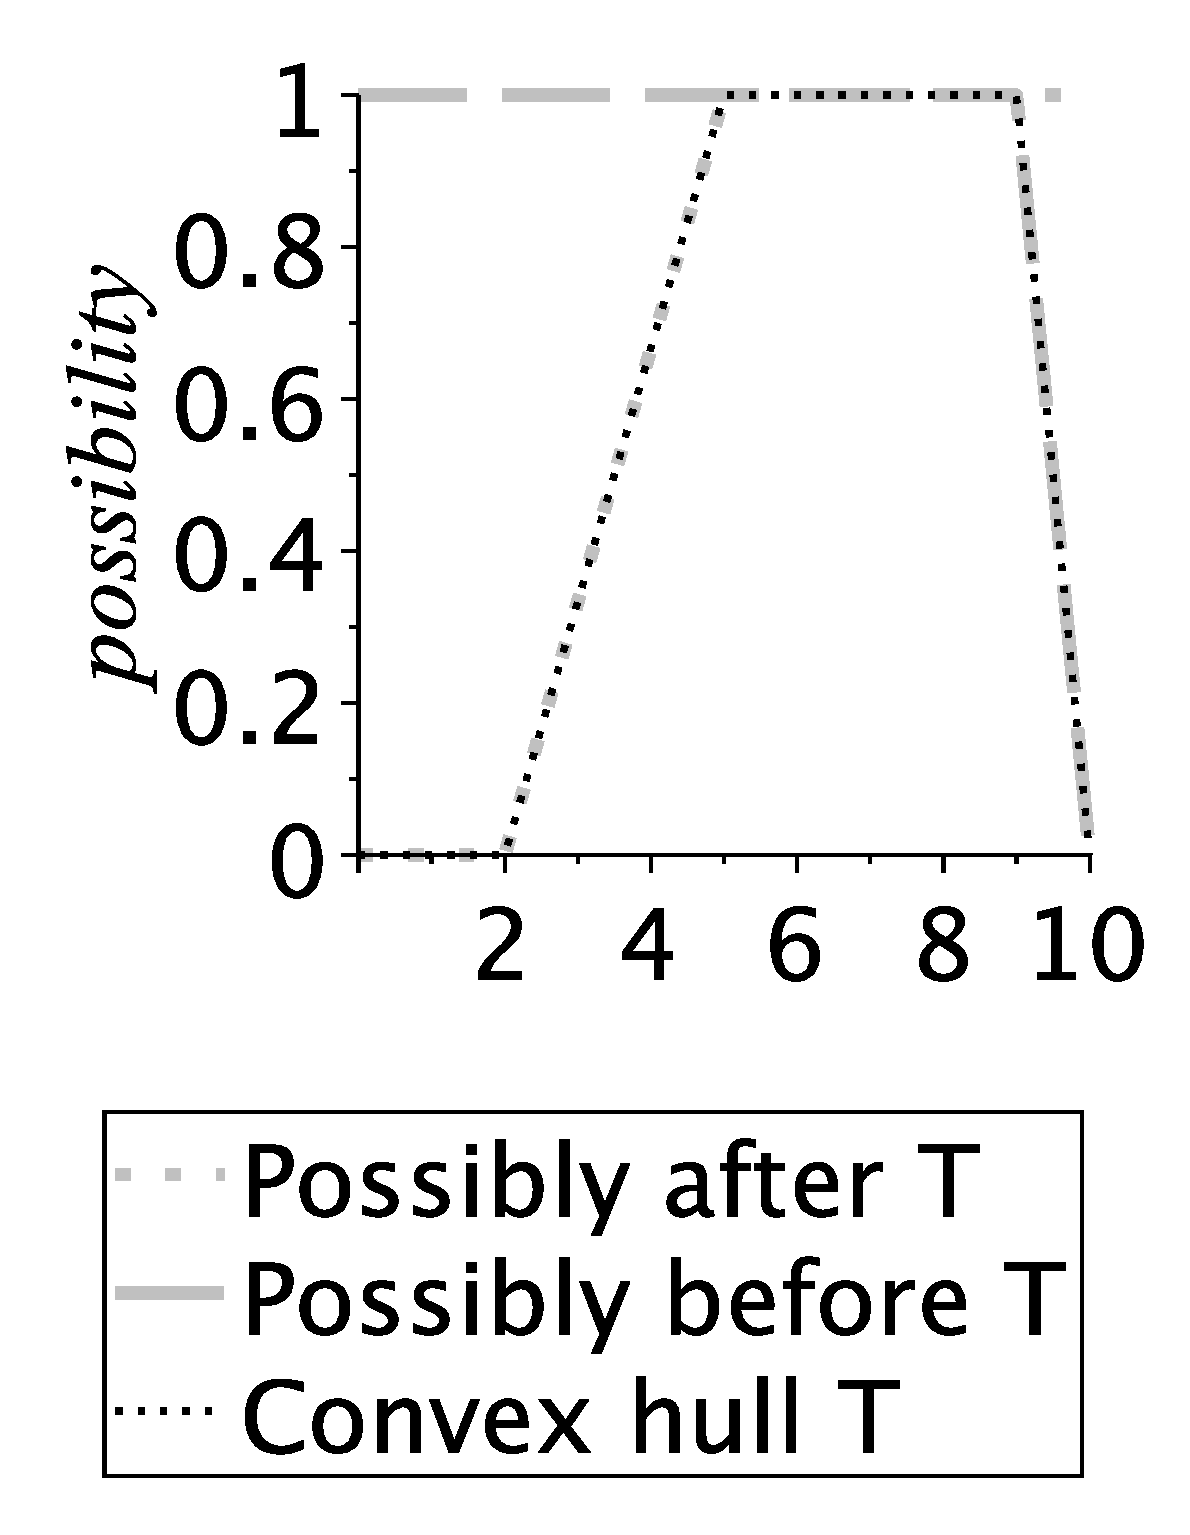
\includegraphics[scale=0.2]{graphs/convexHull/possAfterBefore.eps}
%  \caption{Possibility distributions for  both $u$ possibly greater or equal to $T$ and $u$ possibly smaller or equal to $T$.}
%  \label{fig:convex-hull-pos}
%\end{figure}

%\begin{align}
%\label{eq:ch-possibly-greater}
%\Pos\left(u \geq T\right) & = \sup_{d \leq u} \mu_{T}\left(d\right)  = [2,5,9,+\infty] \\
%\label{eq:ch-possibly-smaller}
%\Pos\left(u \leq T\right) & = \sup_{d \geq u} \mu_{T}\left(d\right)  = [-\infty,5,9,10] 
%\end{align}

%Respectively, the necessity mesaures for a point $u$ w.r.t. the convex hull $T$ are the following (Figure \ref{fig:convex-hull-nec}):

%\begin{align}
%\Nec\left(u \geq T\right) &=  1 - \Pos\left(u \geq T\right) = 1 - \sup_{d \geq u} \mu_{T}\left(d\right) = [9,10,+\infty,+\infty] \\ 
%\Nec\left(u \leq T\right) & = 1 - \Pos\left(u \geq T\right)  = \sup_{d \leq u} \mu_{T}\left(d\right)  = [-\infty,-\infty, 2,5]
%\end{align}

%\begin{figure}[h!]
%  \centering
%  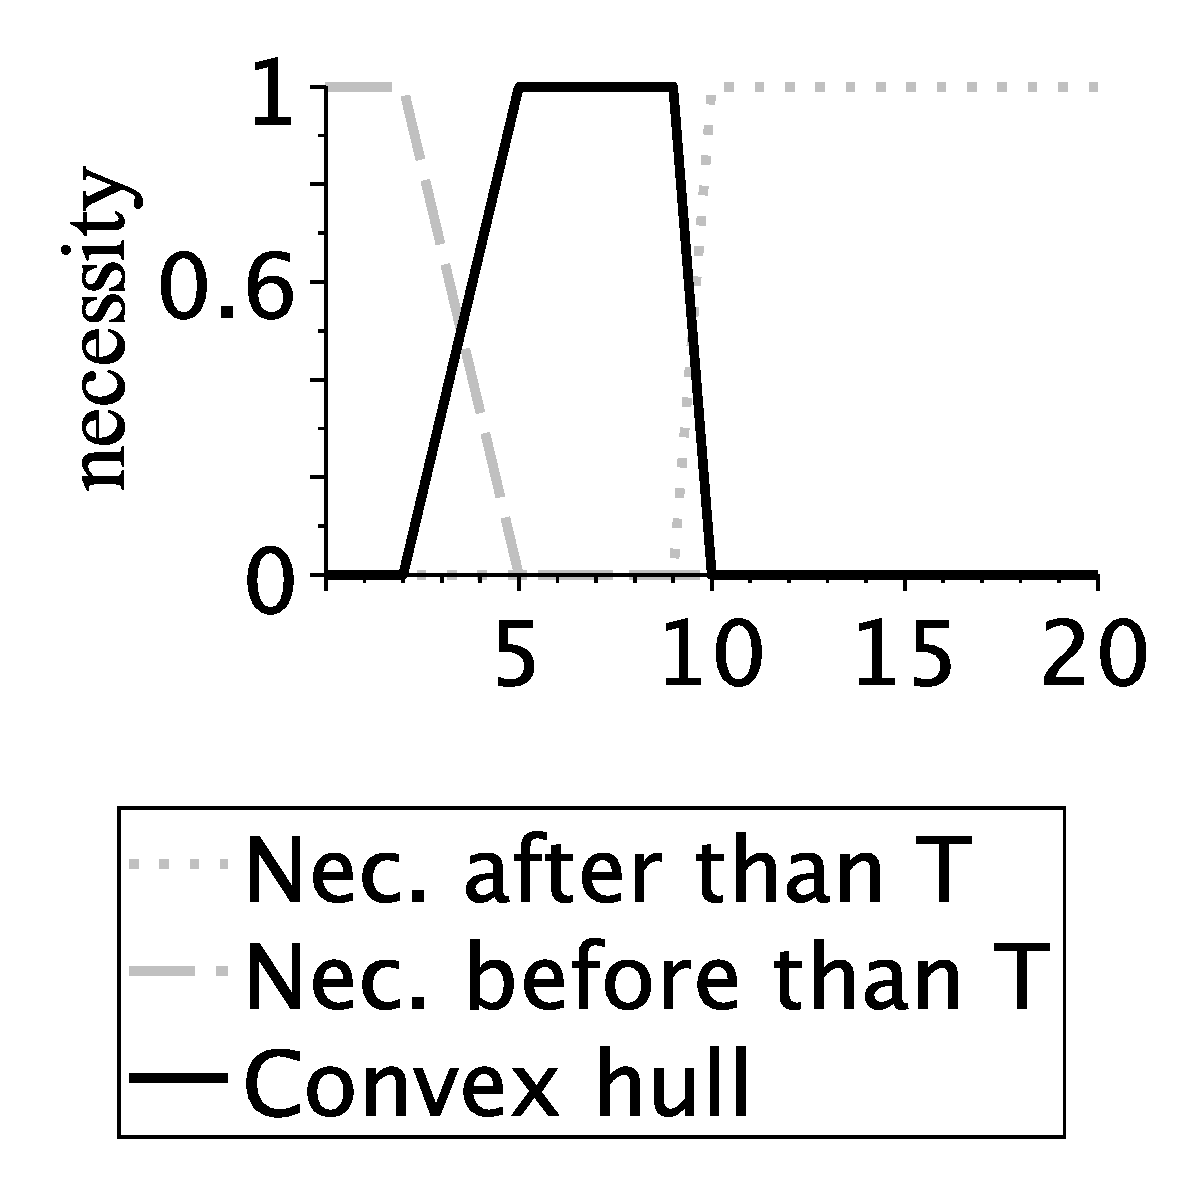
\includegraphics[scale=0.2]{graphs/convexHull/necessity.eps}
%  \caption{Necessity distributions for both $u$ is necessarily greater or equal to $T$ and $u$ is necessarily smaller or equal to $T$.}
%  \label{fig:convex-hull-nec}
%\end{figure}

The membership about an interval $[u,v]$ w.r.t the convex hull $T$ is given by:

\begin{equation}
\label{eq:membership-ch}
\mu_T([u,v]) = \min \left( \mu_T\left(u\right), \mu_T\left(v\right)\right)
\end{equation}


Figure \ref{fig:ch-3d-possibility} shows the 3D plot of the membership function for any interval $[u,v]$ w.r.t. the convex hull $T$ (equation \eqref{eq:membership-ch}). Note that figure Figure \ref{fig:ch-3d-possibility} is equivalent to figure \ref{fig:3d-possibility}. Due to the transformation, it is impossible to obtain a necessity measure.

\begin{figure}[h!]
  \centering
  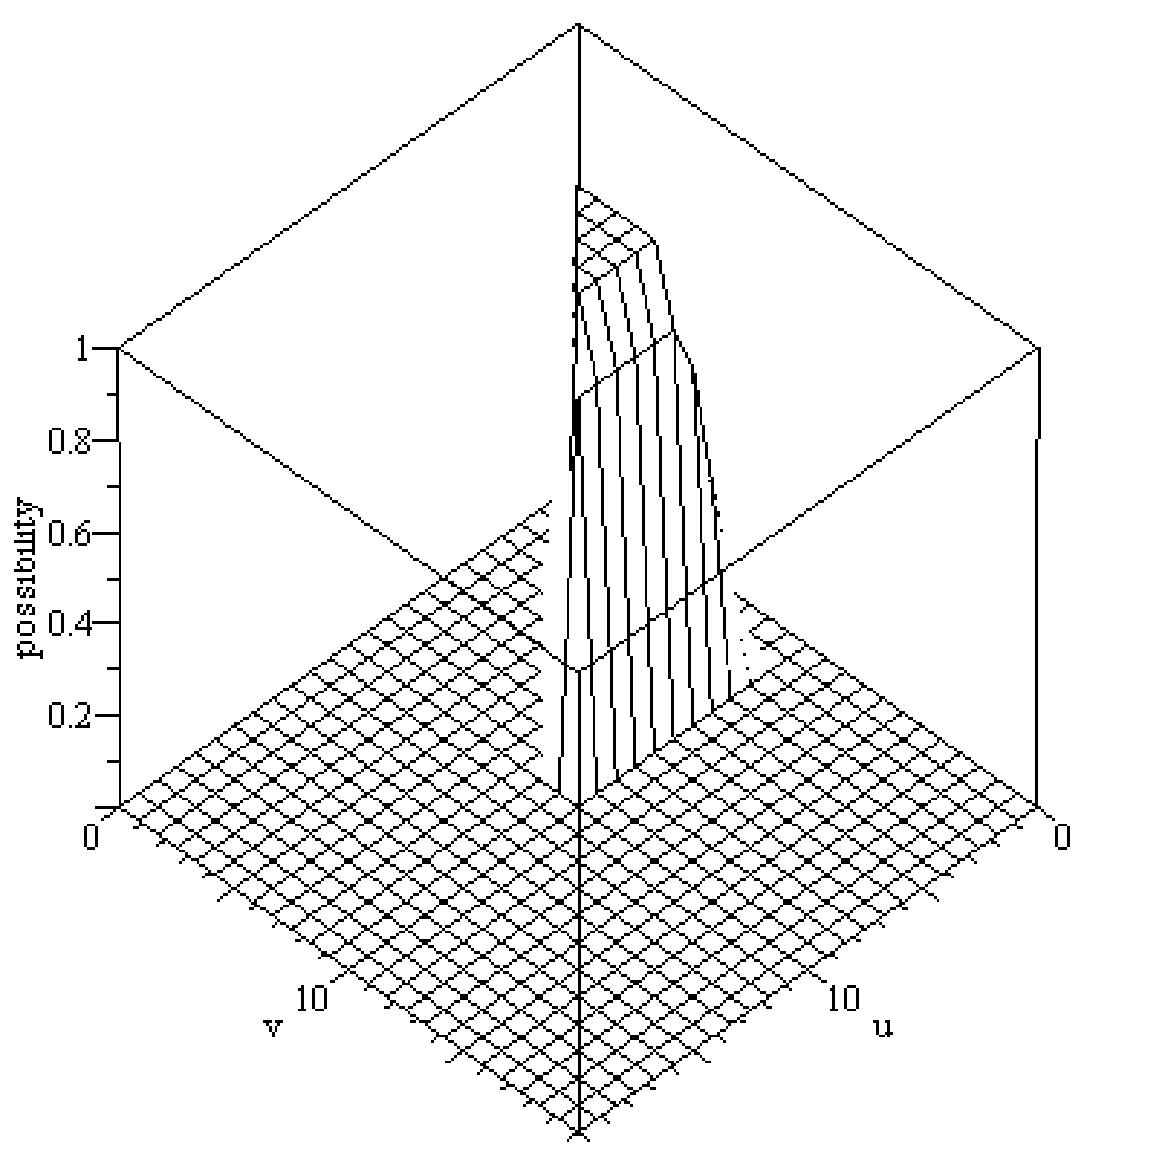
\includegraphics[scale=0.4]{graphs/convexHull/3dpossibility.pdf}
  \caption{Membership function for interval $[u,v]$ w.r.t. the convex hull $T$.}
  \label{fig:ch-3d-possibility}
\end{figure}

%\begin{figure}[h!]
%  \centering
%  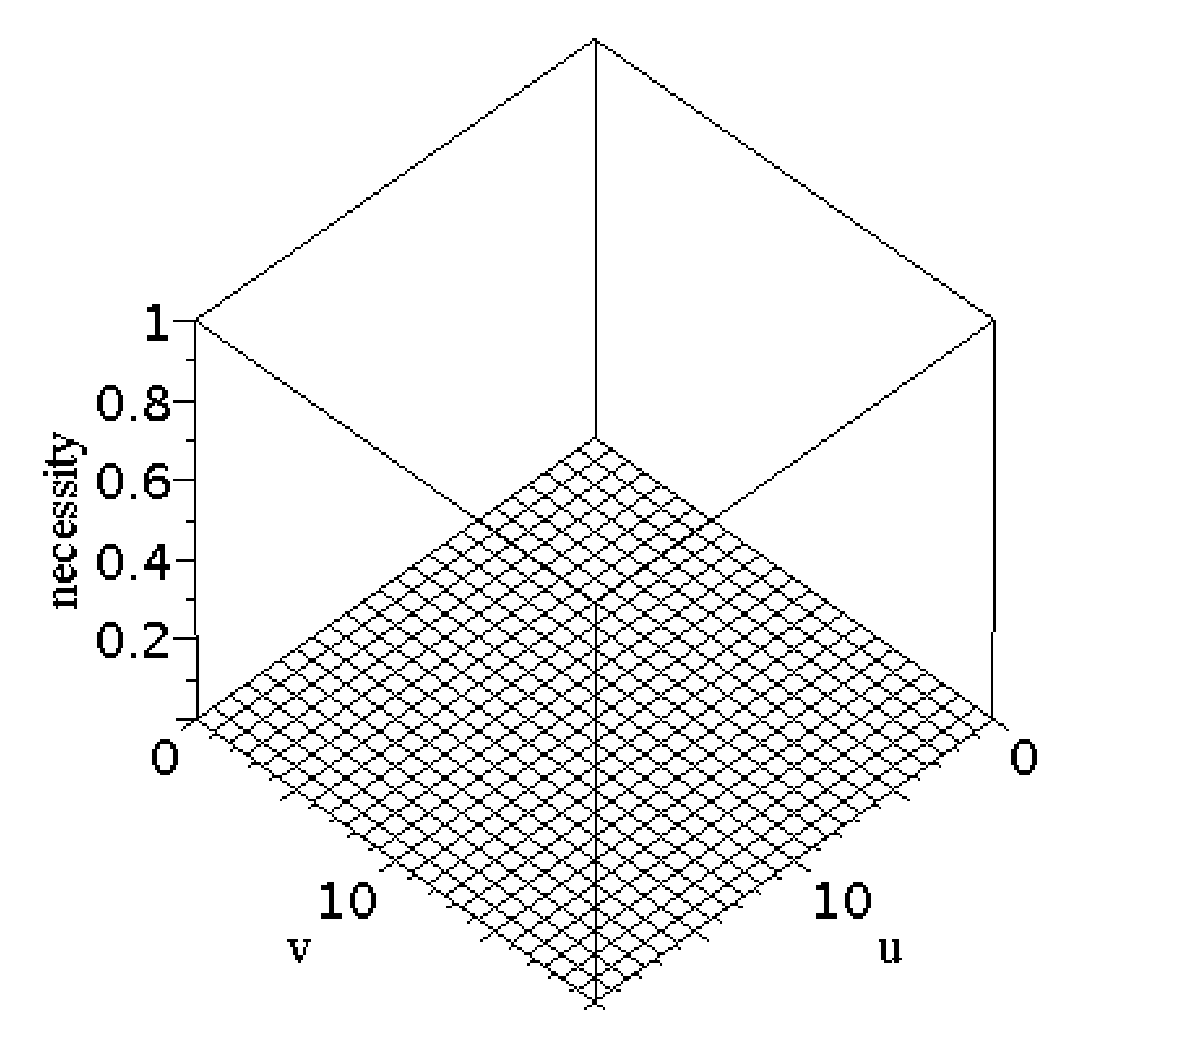
\includegraphics[scale=0.4]{graphs/convexHull/3dnecessity.eps}
%  \caption{Necessity of any interval $[u,v]$ w.r.t. the convex hull $T$.}
%  \label{fig:ch-3d-necessity}
%\end{figure}


%\end{example}








\section{\label{sec:conclusions}CONCLUSIONS AND FUTURE WORK}
The problem of evaluation of sets in the framework of possibility theory has been addressed by Dubois and Prade. They conclude that a correct treatment of sets imply an overly complex possibility distribution. Based on the previous work from the authors, this work is focused on the evaluation of fuzzy temporal interval in the framework of possibility theory. The aim of the paper is to clarify the difference between fuzzy numbers, fuzzy intervals and ill-known intervals. Several proposals can be found in the literature with respect to transforming two fuzzy numbers into a fuzzy interval. We have shown that these techniques are not fully correct in the sense of possibility theory.\\


%Submitted full papers are to be 4 to 6 pages length. Papers must be written on two columns with an overall width of 17.2 cm (8.25 cm each column and 0.7 cm of space between columns). On odd pages, left margin should be of 2.5 cm while the right one should be of 1.3 cm. On even pages, margins are just the contrary (left 1.3 cm, and right 2.5 cm). On all pages, odd and even ones, upper margin should be of 2.5 cm, and lower margin should be of 3.5 cm. Text alignment must be \textit{justify}. The pages must not be numbered.
%
%LaTeX style file (estylf\_en.sty) and the example file
%(estylf2012\_en.tex) are available in the ESTYLF2012 web page.
%
%\section{PRELIMINARIES}
%
%\subsection{SECTIONS AND SUBSECTIONS}
%
%\subsubsection{Subsection}
%All subsections must follow the same format as this one.
%
%\subsection{EQUATIONS}
%All equations must be centered.
%\begin{equation}
%\mu_A = f(a,b,c).
%\end{equation}
%
%\subsection{FIGURES}
%All figures must be centered like Figure~\ref{figure1}. The number and caption of the figure must always appear below the figure.

%\begin{figure}[h]
%\begin{center}
%\includegraphics[width=8cm,height=2.5cm]{estylf2012.jpg}
%\end{center}
%\caption{Example of figure caption.}
%\label{figure1}
%\end{figure}

%\subsection{TABLES}
%All tables must be centered and clear. The number and title always appear above the table (see Table~\ref{table1}).
%
%\begin{table}[ht]
%\begin{center}
%\caption{Example of table title.}
%\label{table1}
%\begin{tabular}{|c|l|} \hline
%\textbf{NAME} & \textbf{DESCRIPTION} \\ \hline
%$A$ & Fuzzy set \\ \hline
%$\mu_{A}$ & Membership function \\
%\hline
%\end{tabular}
%\end{center}
%\end{table}

%\subsection{FOOTNOTES}
%Footnotes must be numbered\footnote{Example of footnote.}, and placed at the bottom of the column where they appear.
%
%\subsection{CITATIONS}
%Citations must include the reference number between square brackets, for example \cite{AlsinaT05}.

\begin{ack}
Part of this research is supported by the grant BES-2009-013805 within the research project TIN2008-02066: \emph{Fuzzy Temporal Information treatment in relational DBMS}.
\end{ack}

\bibliographystyle{acm}
\bibliography{biblio}

%\begin{thebibliography}{99}

%\bibitem{AlsinaT05}
%C. Alsina, E. Trillas: On the symmetric difference of fuzzy sets. \emph{Fuzzy Sets and Systems} 153, pp.~181--194, 2005.
%
%\bibitem{Fishburn73}
%P.C. Fishburn: \emph{Utility Theory for Decision Making}. Wiley, New York, 1970.
%
%\bibitem{Yager03}
%R.R. Yager: E-Z OWA weights. In: \emph{Proceedings of the 10th IFSA World Congress}, Istanbul (Turkey), pp.~39--42, 2003.
%
%\bibitem{Zadeh71}
%L.A. Zadeh: Towards a theory of fuzzy systems. In: R.E. Kalman, N. DeClaris (Eds.), \emph{Aspects of Network and System Theory}, Holt, Rinehart and Winston, New York, pp.~469--490, 1971.

%\end{thebibliography}

%References must be sorted by the author name.

\end{document}
